\documentclass[11pt,a4paper]{article}

% Pacotes essenciais
\usepackage[utf8]{inputenc}
\usepackage[T1]{fontenc}
\usepackage{lmodern}
\usepackage[portuguese]{babel}
\usepackage{graphicx}
\usepackage{amsmath}
\usepackage{amsfonts}
\usepackage{amssymb}
\usepackage{float}
\usepackage{caption}
\usepackage{subcaption}
\usepackage{xcolor}
\usepackage{colortbl}
\usepackage{fancyhdr}
\usepackage{geometry}
\usepackage{titlesec}
\usepackage{lipsum}
\usepackage[alf]{abntex2cite}
\usepackage{booktabs}
\usepackage{array}
\usepackage{enumitem}
\usepackage{tikz}
\usetikzlibrary{shapes.geometric}
\usepackage[hidelinks]{hyperref}

% Definição das cores
\definecolor{headercolor}{HTML}{b11116}
\definecolor{secondarycolor}{HTML}{3a5461}

% Configuração da página
\geometry{
    a4paper,
    top=2.8cm,
    bottom=2.5cm,
    left=2.5cm,
    right=2.5cm,
    headheight=1.2cm,
    headsep=0.5cm
}

% Configuração do cabeçalho
\pagestyle{fancy}
\fancyhf{}
\renewcommand{\headrulewidth}{0pt}
\renewcommand{\footrulewidth}{0.5pt}

\fancyhead[L]{%
    \begin{tikzpicture}[remember picture, overlay]
        \fill[headercolor] (current page.north west) rectangle ([yshift=-1.2cm]current page.north east);
        \node[anchor=west, inner sep=0pt] at ([xshift=1cm, yshift=-0.6cm]current page.north west) 
            {
\includegraphics[height=0.8cm]{imgs/base/fatec-rgt.png}};
        \node[anchor=east, inner sep=0pt] at ([xshift=-1cm, yshift=-0.6cm]current page.north east) 
            {
\includegraphics[height=0.9cm]{imgs/base/cps-logo.png}};
        \node[anchor=east, inner sep=0pt] at ([xshift=-2.8cm, yshift=-0.6cm]current page.north east) 
            {
\includegraphics[height=1.05cm]{imgs/base/governo-sp-secretaria-logo.png}};
    \end{tikzpicture}
}

\fancyfoot[L]{\footnotesize\textcolor{secondarycolor}{Faculdade de Tecnologia do Estado de São Paulo\\ fatecregistro.cps.sp.gov.br}}
\fancyfoot[R]{\thepage}

% Configuração dos títulos das seções
\titleformat{\section}
    {\normalfont\large\bfseries\color{secondarycolor}}
    {\thesection}{1em}{}

\titleformat{\subsection}
    {\normalfont\normalsize\bfseries\color{secondarycolor}}
    {\thesubsection}{1em}{}

\begin{document}

% ===== CAPA =====
\begin{titlepage}
    \centering
    
    % Logos no topo
    \begin{tikzpicture}[remember picture, overlay]
        \fill[headercolor] (current page.north west) rectangle ([yshift=-1.2cm]current page.north east);
        \node[anchor=west, inner sep=0pt] at ([xshift=1cm, yshift=-0.6cm]current page.north west) 
            {
\includegraphics[height=0.8cm]{imgs/base/fatec-rgt.png}};
        \node[anchor=east, inner sep=0pt] at ([xshift=-1cm, yshift=-0.6cm]current page.north east) 
            {
\includegraphics[height=0.9cm]{imgs/base/cps-logo.png}};
        \node[anchor=east, inner sep=0pt] at ([xshift=-2.8cm, yshift=-0.6cm]current page.north east) 
            {
\includegraphics[height=1.05cm]{imgs/base/governo-sp-secretaria-logo.png}};
    \end{tikzpicture}
    
    \vspace*{3.5cm}
    
    % Nome da faculdade
    {\normalsize FACULDADE DE TECNOLOGIA DO ESTADO DE SÃO PAULO\par}
    \vspace{0.5cm}
    
    % Curso
    {\normalsize DESENVOLVIMENTO DE SOFTWARE MULTIPLATAFORMA\par}
    
    \vspace{4cm}
    
    % Artefatos do Projeto de Software
    {\normalsize ARTEFATOS DO PROJETO DE SOFTWARE\par}
    
    \vspace{0.3cm}
    
    % Nome do projeto
    {\normalsize Detecção de fungos parasitas em cogumelos por meio de Aprendizagem Profunda\par}
    
    \vspace{3cm}
    
    % Autores
    {\normalsize
    Andrei Lucas\\
    Ricardo Estevam\\
    Leandro Sueoka\\
    Lucas Barros\\
    Érlon Viana
    }
    
    \vfill
    
    % Rodapé
    {\small Registro -- SP\\
    2026}
    
\end{titlepage}

% Força o cabeçalho em todas as páginas
\pagestyle{fancy}

% ===== SUMÁRIO =====
\tableofcontents
\newpage

% ===== NOTA IMPORTANTE =====
\section*{Introdução Artefatos de Software}

\noindent Este documento apresenta os principais artefatos do projeto de software Selene, demonstrando sua estrutura, organização e os elementos utilizados ao longo do desenvolvimento do sistema.

\subsection*{Lista de Artefatos e suas Finalidades}

\begin{itemize}
    \item \textbf{CANVAS:} Modelagem de negócio e proposta estratégica do Selene
    \item \textbf{SWOT:} Análise estratégica de forças, fraquezas, oportunidades e ameaças do projeto
    \item \textbf{UX/UI:} Planejamento da interface e experiência do usuário do sistema
    \item \textbf{Website:} Estrutura, navegação e especificações técnicas da plataforma web
    \item \textbf{Diagramas UML:} Representação visual da arquitetura e funcionamento do sistema
    \item \textbf{DevOps:} Automação, integração contínua e gerenciamento da infraestrutura do Selene
\end{itemize}

\vspace{0.5cm}
\noindent\rule{\textwidth}{0.5pt}

\newpage

% ===== CANVAS =====
\section{CANVAS: Modelo de Negócio e Estratégia}

O Business Model Canvas do projeto de software Selene apresenta, de forma visual e estratégica, a estrutura do modelo de negócios do sistema, destacando os nove blocos fundamentais que representam as principais áreas envolvidas na proposta, operação, relacionamento com usuários e geração de valor da solução.

\subsection{Modelo Estruturado Canvas}

\begin{figure}[H]
    \centering
    
    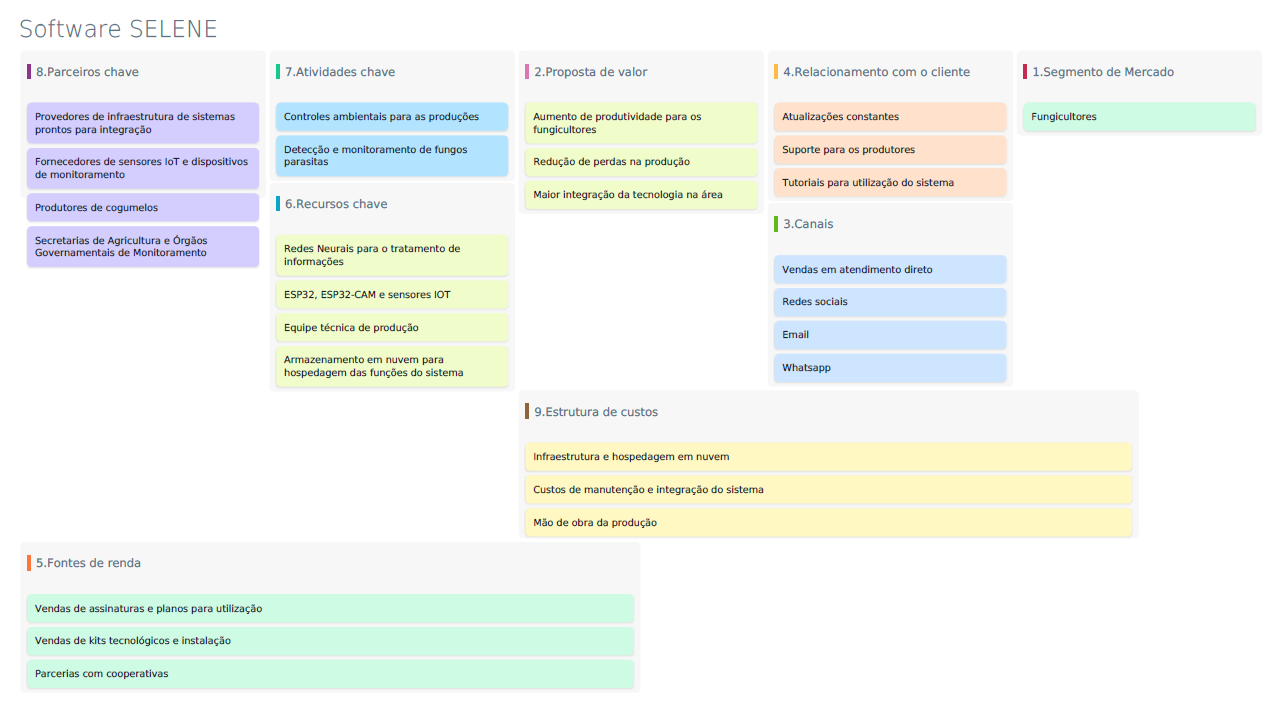
\includegraphics[
        width=0.8\textwidth,
        height=0.8\textheight,
        keepaspectratio
    ]{imgs/img_002.png}
    
    \caption{Business Model Canvas do Projeto Selene}
    \label{fig:canvas}
\end{figure}

% ===== SWOT =====
\section{SWOT: Análise Estratégica}

A Análise SWOT (Strengths, Weaknesses, Opportunities, Threats), também conhecida como FOFA (Forças, Oportunidades, Fraquezas e Ameaças), é uma ferramenta estratégica utilizada para identificar fatores internos e externos que podem influenciar o desenvolvimento do projeto Selene. Por meio dessa análise, são avaliadas as principais forças e fraquezas do sistema, bem como as oportunidades e ameaças presentes no ambiente em que a solução está inserida, contribuindo para o planejamento e tomada de decisões do projeto.

\subsection{Modelo Estruturado Análise SWOT}

\begin{figure}[H]
    \centering
    
    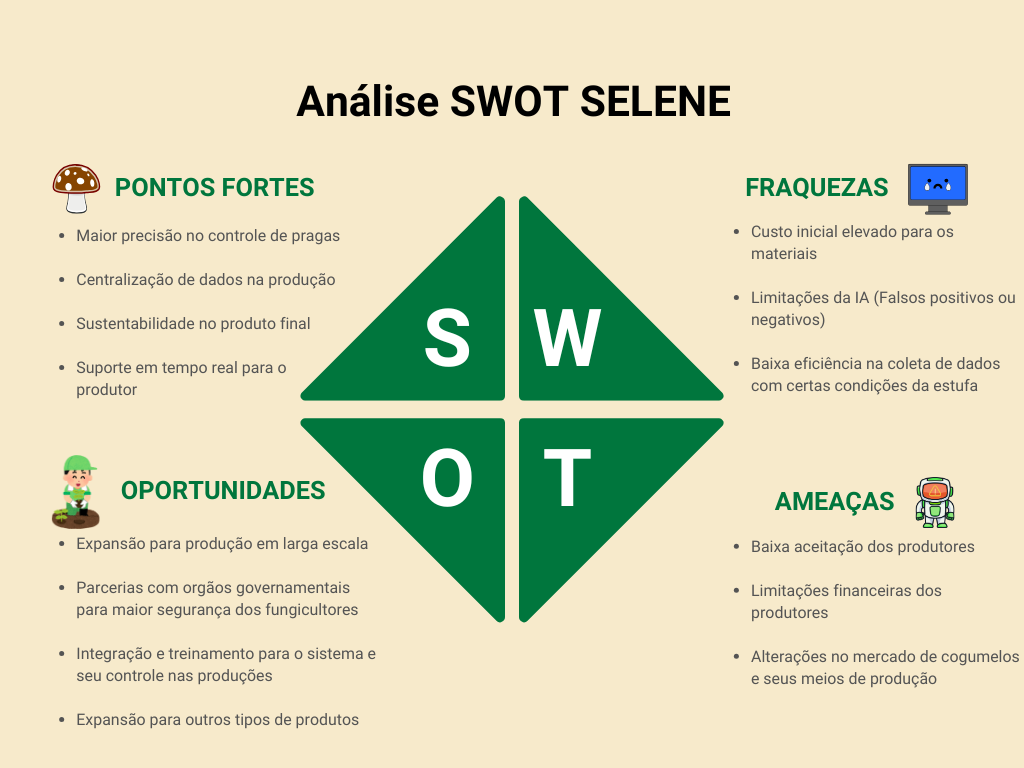
\includegraphics[
        width=0.6\textwidth,
        height=0.6\textheight,
        keepaspectratio
    ]{imgs/img_003.png}
    
    \caption{Análise SWOT do Projeto Selene}
    \label{fig:swot}
\end{figure}

\subsection{Recomendações Estratégicas}

Com base na análise SWOT, as principais estratégias devem focar em:
\begin{itemize}
    \item \textbf{Forças + Oportunidades:} Utilizar a precisão no controle de pragas, a centralização de dados e o suporte em tempo real para expandir o sistema em produções de larga escala e fortalecer parcerias no setor agrícola.
    \item \textbf{Forças + Ameaças:} Destacar a sustentabilidade e a eficiência do sistema Selene para aumentar a aceitação dos produtores e reduzir os impactos das limitações financeiras do mercado.
    \item \textbf{Fraquezas + Oportunidades:} Buscar incentivos, treinamentos e parcerias estratégicas para minimizar os custos iniciais e aprimorar a utilização da inteligência artificial no sistema.
    \item \textbf{Fraquezas + Ameaças:} Desenvolver melhorias contínuas na coleta de dados das estufas e criar estratégias de suporte técnico para reduzir falhas operacionais e dificuldades de adoção pelos produtores.
\end{itemize}

% ===== UX/UI =====
\section{UX/UI: Design de Interface e Experiência do Usuário}

UX (User Experience) e UI (User Interface) são áreas fundamentais utilizadas no desenvolvimento do projeto Selene para garantir uma navegação intuitiva, acessível e eficiente. O UX está relacionado à experiência do usuário durante a utilização do sistema, focando na usabilidade e facilidade de interação. Já o UI envolve os elementos visuais da plataforma, como cores, botões, tipografia, ícones e organização das telas, contribuindo para uma interface mais clara e agradável ao produtor.

\subsection{Mockups e Protótipos}

Os artefatos de UX/UI do projeto Selene incluem demonstrações de protótipos de baixa fidelidade (wireframes) e de alta fidelidade, utilizados para representar visualmente a estrutura, navegação e aparência final das interfaces do sistema.

\begin{figure}[H]
\centering
\begin{minipage}{0.45\textwidth}
    \centering
    \fbox{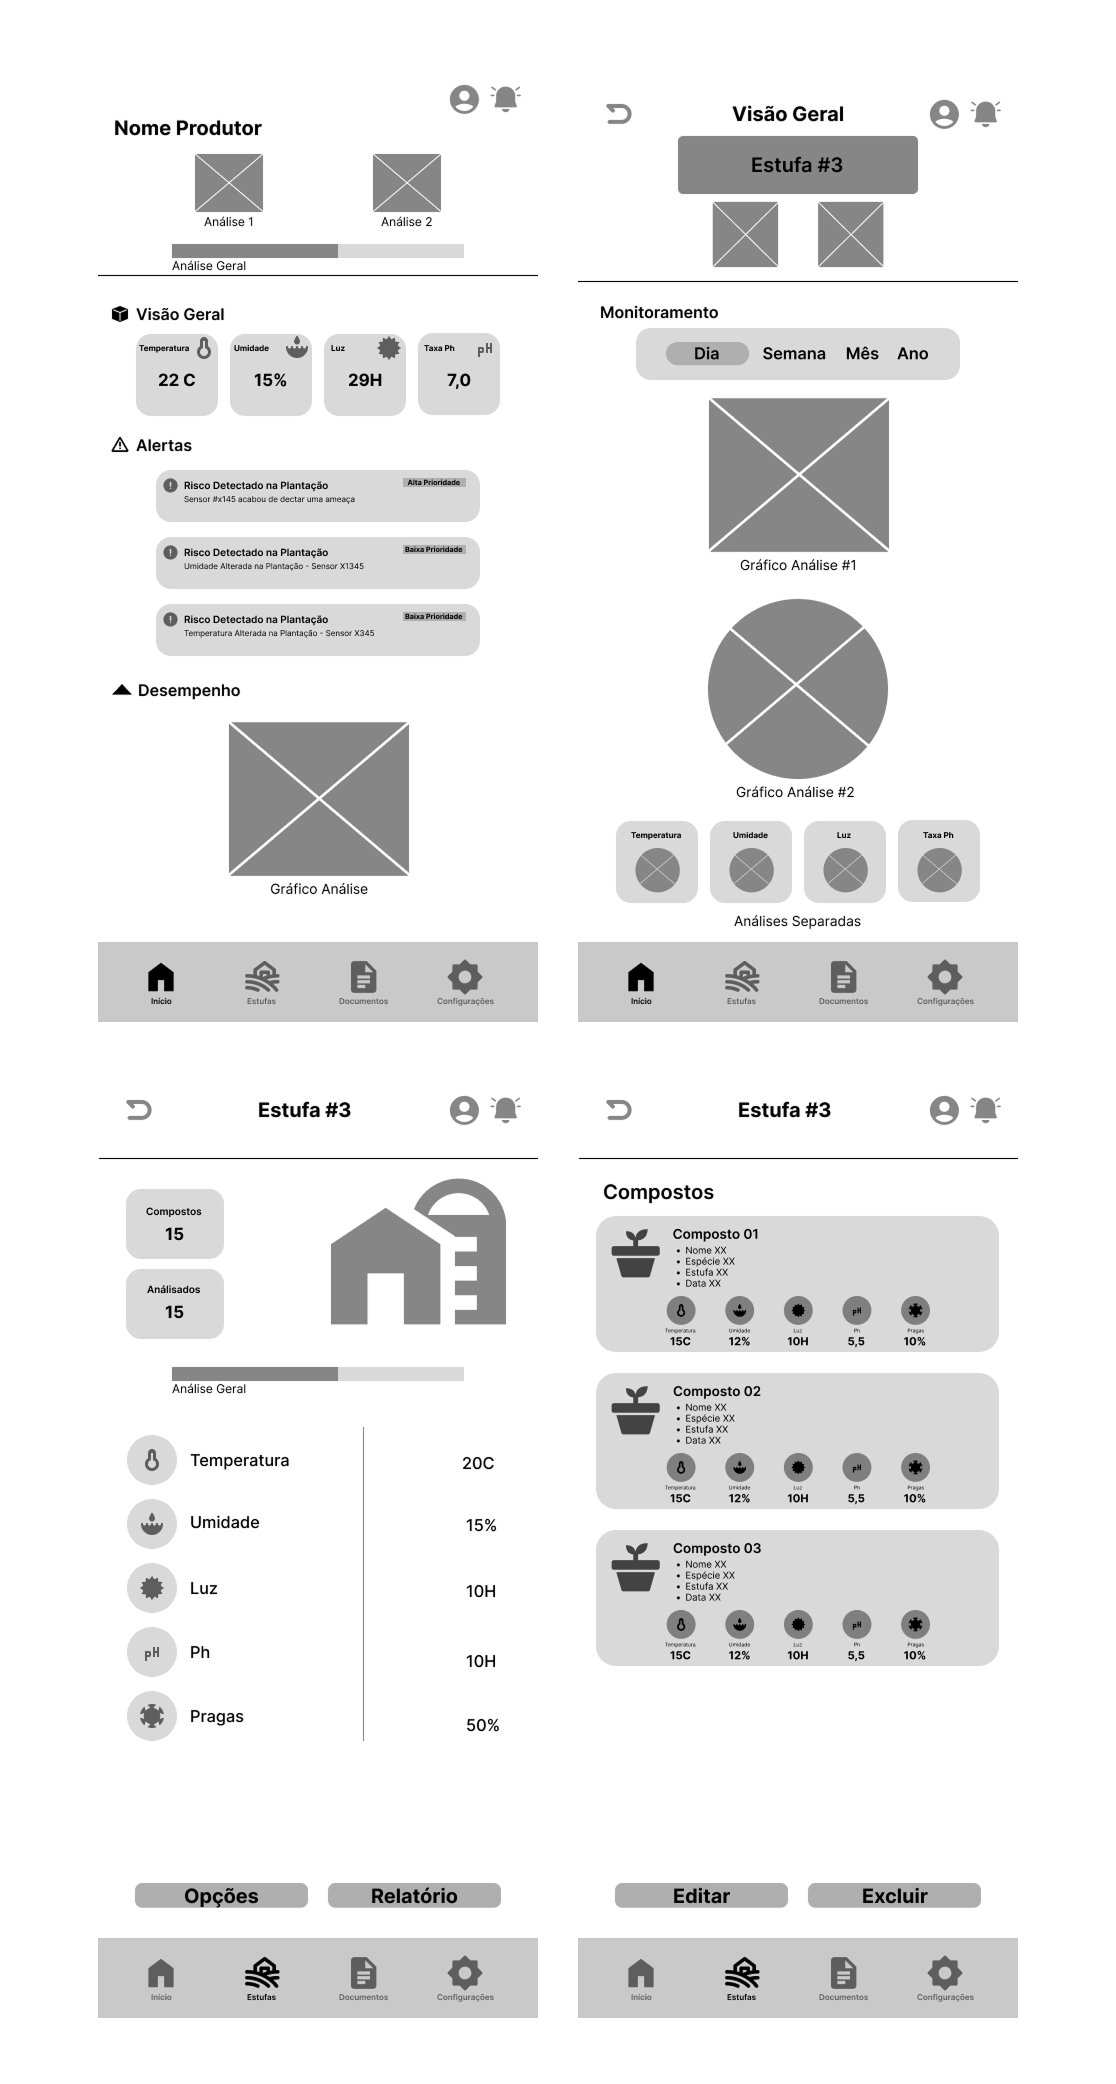
\includegraphics[width=0.9\textwidth]{imgs/Frame 1.png}}
    \caption{Modelo Wireframe Core - Selene}
    \label{fig:wireframe}
\end{minipage}
\hfill
\begin{minipage}{0.45\textwidth}
    \centering
    \fbox{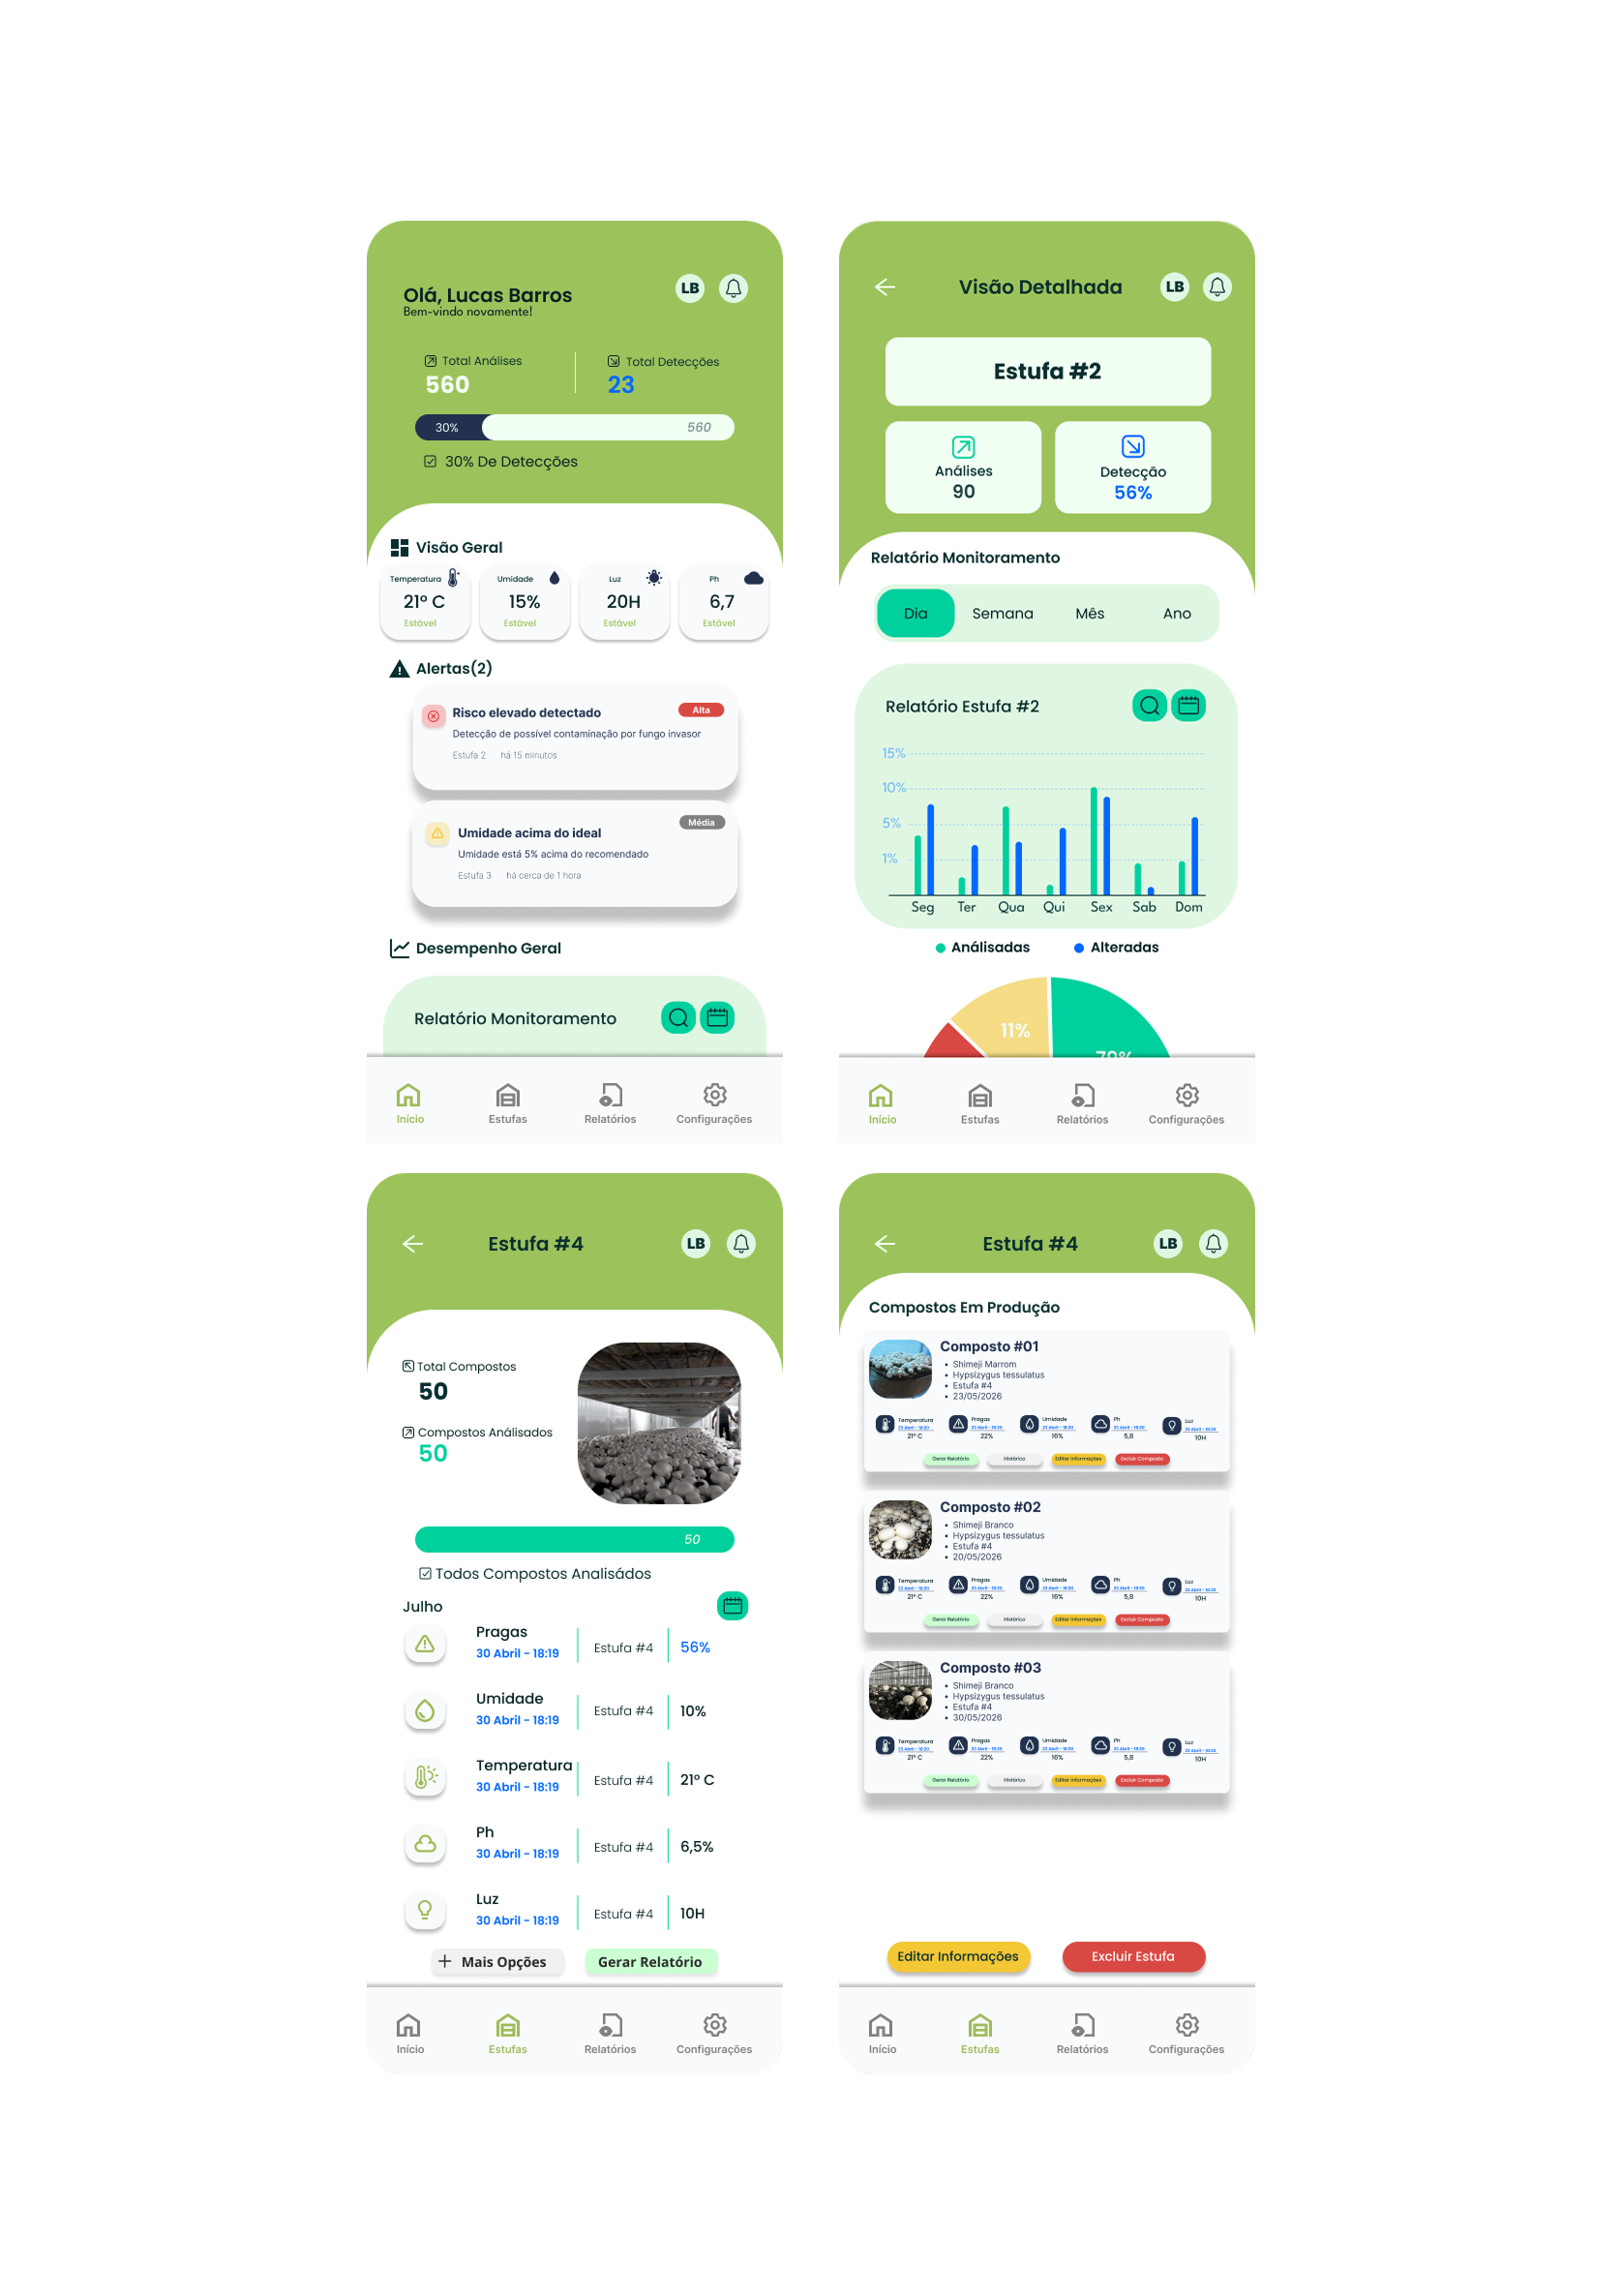
\includegraphics[width=0.9\textwidth]{imgs/Frame 2.png}}
    \caption{Modelo de alta fidelidade Core - Selene}
    \label{fig:mockup}
\end{minipage}
\end{figure}

\subsection{Guia de Estilos}

A seguir, mostra-se o design system utilizado no projeto Selene, apresentando os padrões visuais, componentes de interface, tipografia, paleta de cores, ícones e demais elementos que garantem consistência e identidade visual ao sistema.

\begin{table}[H]
\centering
\caption{Design System -- Projeto Selene}
\label{tab:designsystem}
\renewcommand{\arraystretch}{1.3}
\small

\begin{tabular}{|p{3.5cm}|p{9.5cm}|}
\hline
\textbf{Elemento} & \textbf{Descrição} \\
\hline

\textbf{Identidade Visual} &
Logo principal nas versões verde e azul escuro, incluindo aplicações horizontais e ícones reduzidos. \\
\hline

\textbf{Tipografia} &
Fontes utilizadas: Poppins, Inter e Open Sans. \\
\hline

\textbf{Paleta de Cores} &
Cinza Médio (\texttt{\#818181}), 
Preto (\texttt{\#000000}), 
Branco (\texttt{\#FFFFFF}), 
Verde Água (\texttt{\#00D09E}), 
Azul Claro (\texttt{\#6DB6FE}), 
Verde Claro (\texttt{\#CBFFD2}), 
Verde Suave (\texttt{\#DFF7E2}), 
Cinza Esverdeado (\texttt{\#F1FFF3}), 
Azul Primário (\texttt{\#0068FF}), 
Verde Lima (\texttt{\#9CC35B}), 
Azul Escuro (\texttt{\#3C4A64}), 
Cinza Claro (\texttt{\#F8FAFC}), 
Vermelho Suave (\texttt{\#D94944}), 
Vermelho Alerta (\texttt{\#F43434}), 
Amarelo Destaque (\texttt{\#F4C734}) e 
Cinza Neutro (\texttt{\#F1F1F1}). \\
\hline

\textbf{Botões} &
Botões padronizados para ações principais e secundárias, incluindo estados normal, hover, ativo e desabilitado. \\
\hline

\textbf{Ícones} &
Conjunto de ícones para navegação, gráficos, funcionalidades do sistema e componentes administrativos. \\
\hline

\textbf{Componentes} &
Elementos reutilizáveis como menus, cartões, gráficos, indicadores e navegação lateral. \\
\hline

\textbf{Estilo Visual} &
Interface moderna, minimalista e responsiva, priorizando acessibilidade e usabilidade. \\
\hline

\end{tabular}
\end{table}

% ===== WEBSITE =====
\section{Website: Estrutura e Especificações Técnicas Web}

Esta seção apresenta o website institucional/portfólio da equipe responsável pelo desenvolvimento do projeto Selene. O site tem como objetivo apresentar os integrantes da equipe, os projetos desenvolvidos, competências técnicas, tecnologias utilizadas e informações de contato relacionadas ao sistema.

\subsection{Mapa do Site da Equipe}

O mapa do site (sitemap) do projeto Selene apresenta a hierarquia e a organização das páginas do website institucional da equipe, demonstrando a estrutura de navegação, divisão de conteúdos e acesso às principais seções da plataforma.

\begin{figure}[H]
    \centering
    
    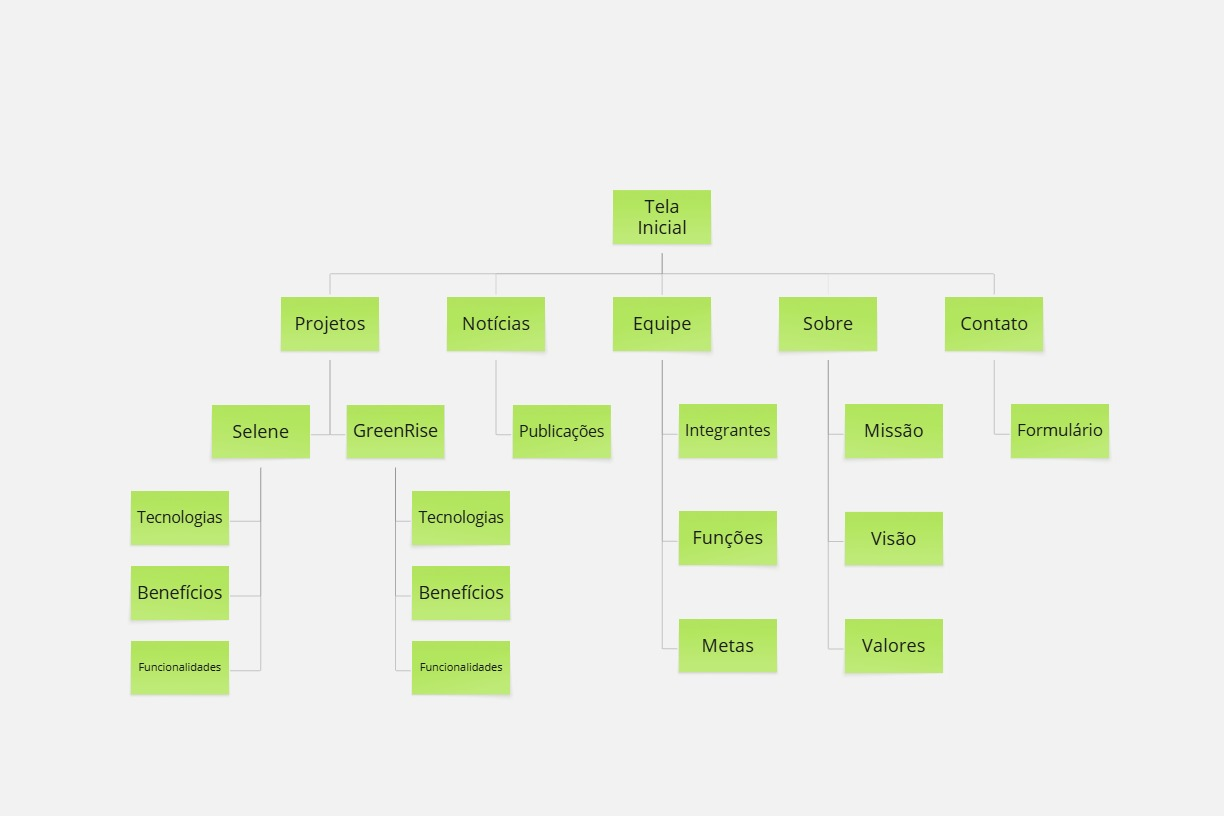
\includegraphics[
        width=0.6\textwidth,
        height=0.6\textheight,
        keepaspectratio
    ]{imgs/img_004.jpg}
    
    \caption{Sitemap do Projeto Selene}
    \label{fig:sitemap}
\end{figure}

\subsection{Conteúdo das Páginas}

\textbf{Páginas principais do site da equipe:}

\begin{itemize}
    \item \textbf{Tela Inicial:} A página inicial apresenta uma visão geral do Projeto Ceres, destacando os principais projetos desenvolvidos, informações institucionais e acesso rápido às demais áreas do site. Seu objetivo é fornecer uma navegação intuitiva e uma introdução ao propósito da plataforma.
    \item \textbf{Sobre:} A seção sobre apresenta a identidade do Projeto Ceres, incluindo missão, visão, valores e metas institucionais, demonstrando os objetivos e princípios que orientam o desenvolvimento das soluções.
    \item \textbf{Equipe:} A página da equipe apresenta os integrantes responsáveis pelo desenvolvimento do projeto, destacando funções, responsabilidades e participação de cada membro na construção das soluções.
    \item \textbf{Projetos:} A seção de projetos reúne as soluções desenvolvidas pela equipe no contexto do Projeto Ceres, apresentando sistemas e iniciativas voltadas à inovação, tecnologia e sustentabilidade. Nessa área, os usuários podem visualizar informações sobre funcionalidades, benefícios e tecnologias utilizadas em cada projeto desenvolvido.
    \item \textbf{Notícias:} A página de notícias disponibiliza publicações, atualizações e conteúdos relacionados ao Projeto Ceres, permitindo acompanhar novidades, eventos e informações relevantes sobre os projetos desenvolvidos.
    \item \textbf{Contato:} A seção de contato disponibiliza um formulário para comunicação entre usuários e a equipe do projeto, permitindo envio de dúvidas, sugestões e solicitações de informações.
\end{itemize}

\subsection{Especificações Técnicas do Site da Equipe}

\begin{table}[H]
\centering
\caption{Stack Tecnológica do Website da Equipe}
\label{tab:stack-web}
\renewcommand{\arraystretch}{1.3}
\small

\begin{tabular}{|p{3cm}|p{3.5cm}|p{7cm}|}
\hline
\textbf{Camada} & \textbf{Tecnologia} & \textbf{Descrição} \\
\hline

Estrutura & HTML5 & Estrutura semântica e acessível do website. \\
\hline

Estilização & CSS3 & Estilo visual, layout responsivo e animações da interface. \\
\hline

Interatividade & JavaScript (Vanilla) & Funcionalidades dinâmicas e interatividade do sistema. \\
\hline

Hospedagem & Vercel & Plataforma de hospedagem e deploy contínuo da aplicação. \\
\hline

Tipografia & Google Fonts (Montserrat) & Fonte moderna, legível e padronizada para a identidade visual. \\
\hline

\end{tabular}
\end{table}

% ===== DIAGRAMAS UML =====
\section{Diagramas UML: Modelagem Visual do Sistema}

A Unified Modeling Language (UML) é uma linguagem de modelagem visual utilizada no projeto Selene para especificar, visualizar e documentar os principais artefatos do sistema de software. Por meio da UML, são representadas estruturas, comportamentos e interações do sistema, auxiliando na organização e compreensão do desenvolvimento da aplicação.

\subsection{Diagrama de Casos de Uso}

O diagrama de casos de uso do projeto Selene representa as principais funcionalidades do sistema sob a perspectiva dos usuários, demonstrando as interações entre os atores e os recursos.

\begin{figure}[H]
    \centering
    
    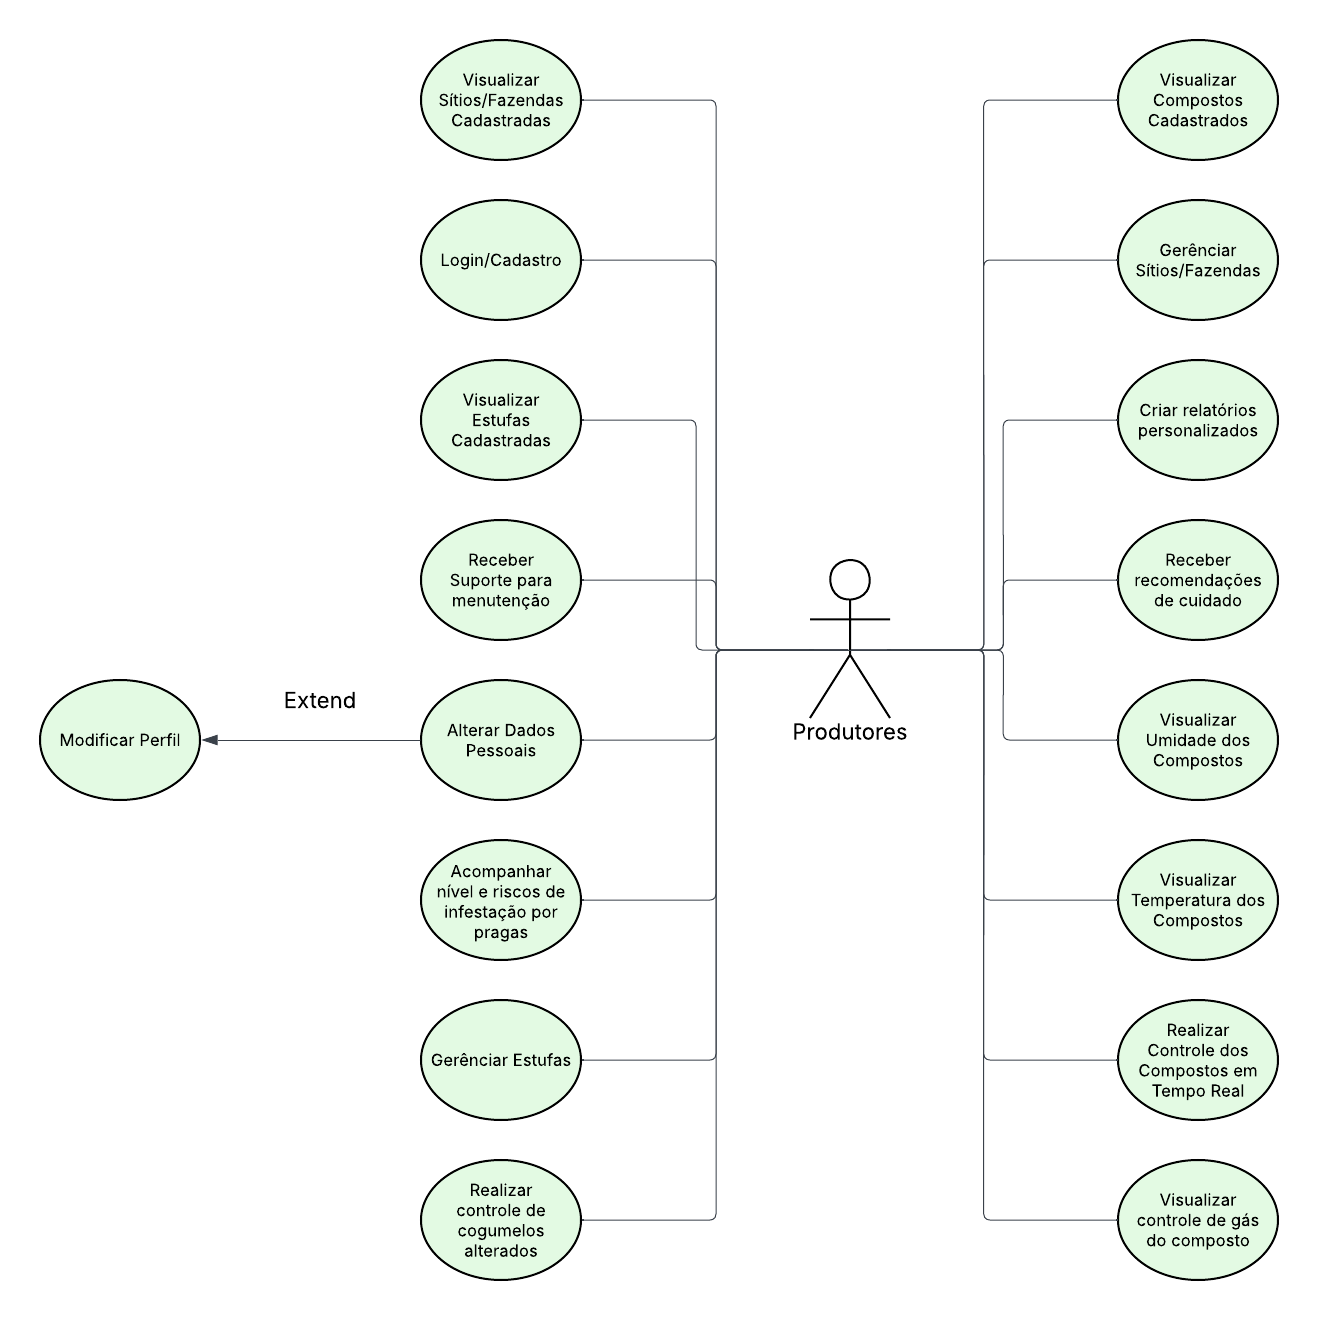
\includegraphics[
        width=0.7\textwidth,
        height=0.7\textheight,
        keepaspectratio
    ]{imgs/img_006.png}
    
    \caption{Diagrama de Casos de Uso -- Selene}
    \label{fig:caso-uso}
\end{figure}

\subsection{Diagrama de Classes}

O diagrama de classes apresenta a estrutura estática do sistema, descrevendo as principais classes, atributos, métodos e os relacionamentos existentes entre os componentes da aplicação.

\begin{figure}[H]
    \centering
    
    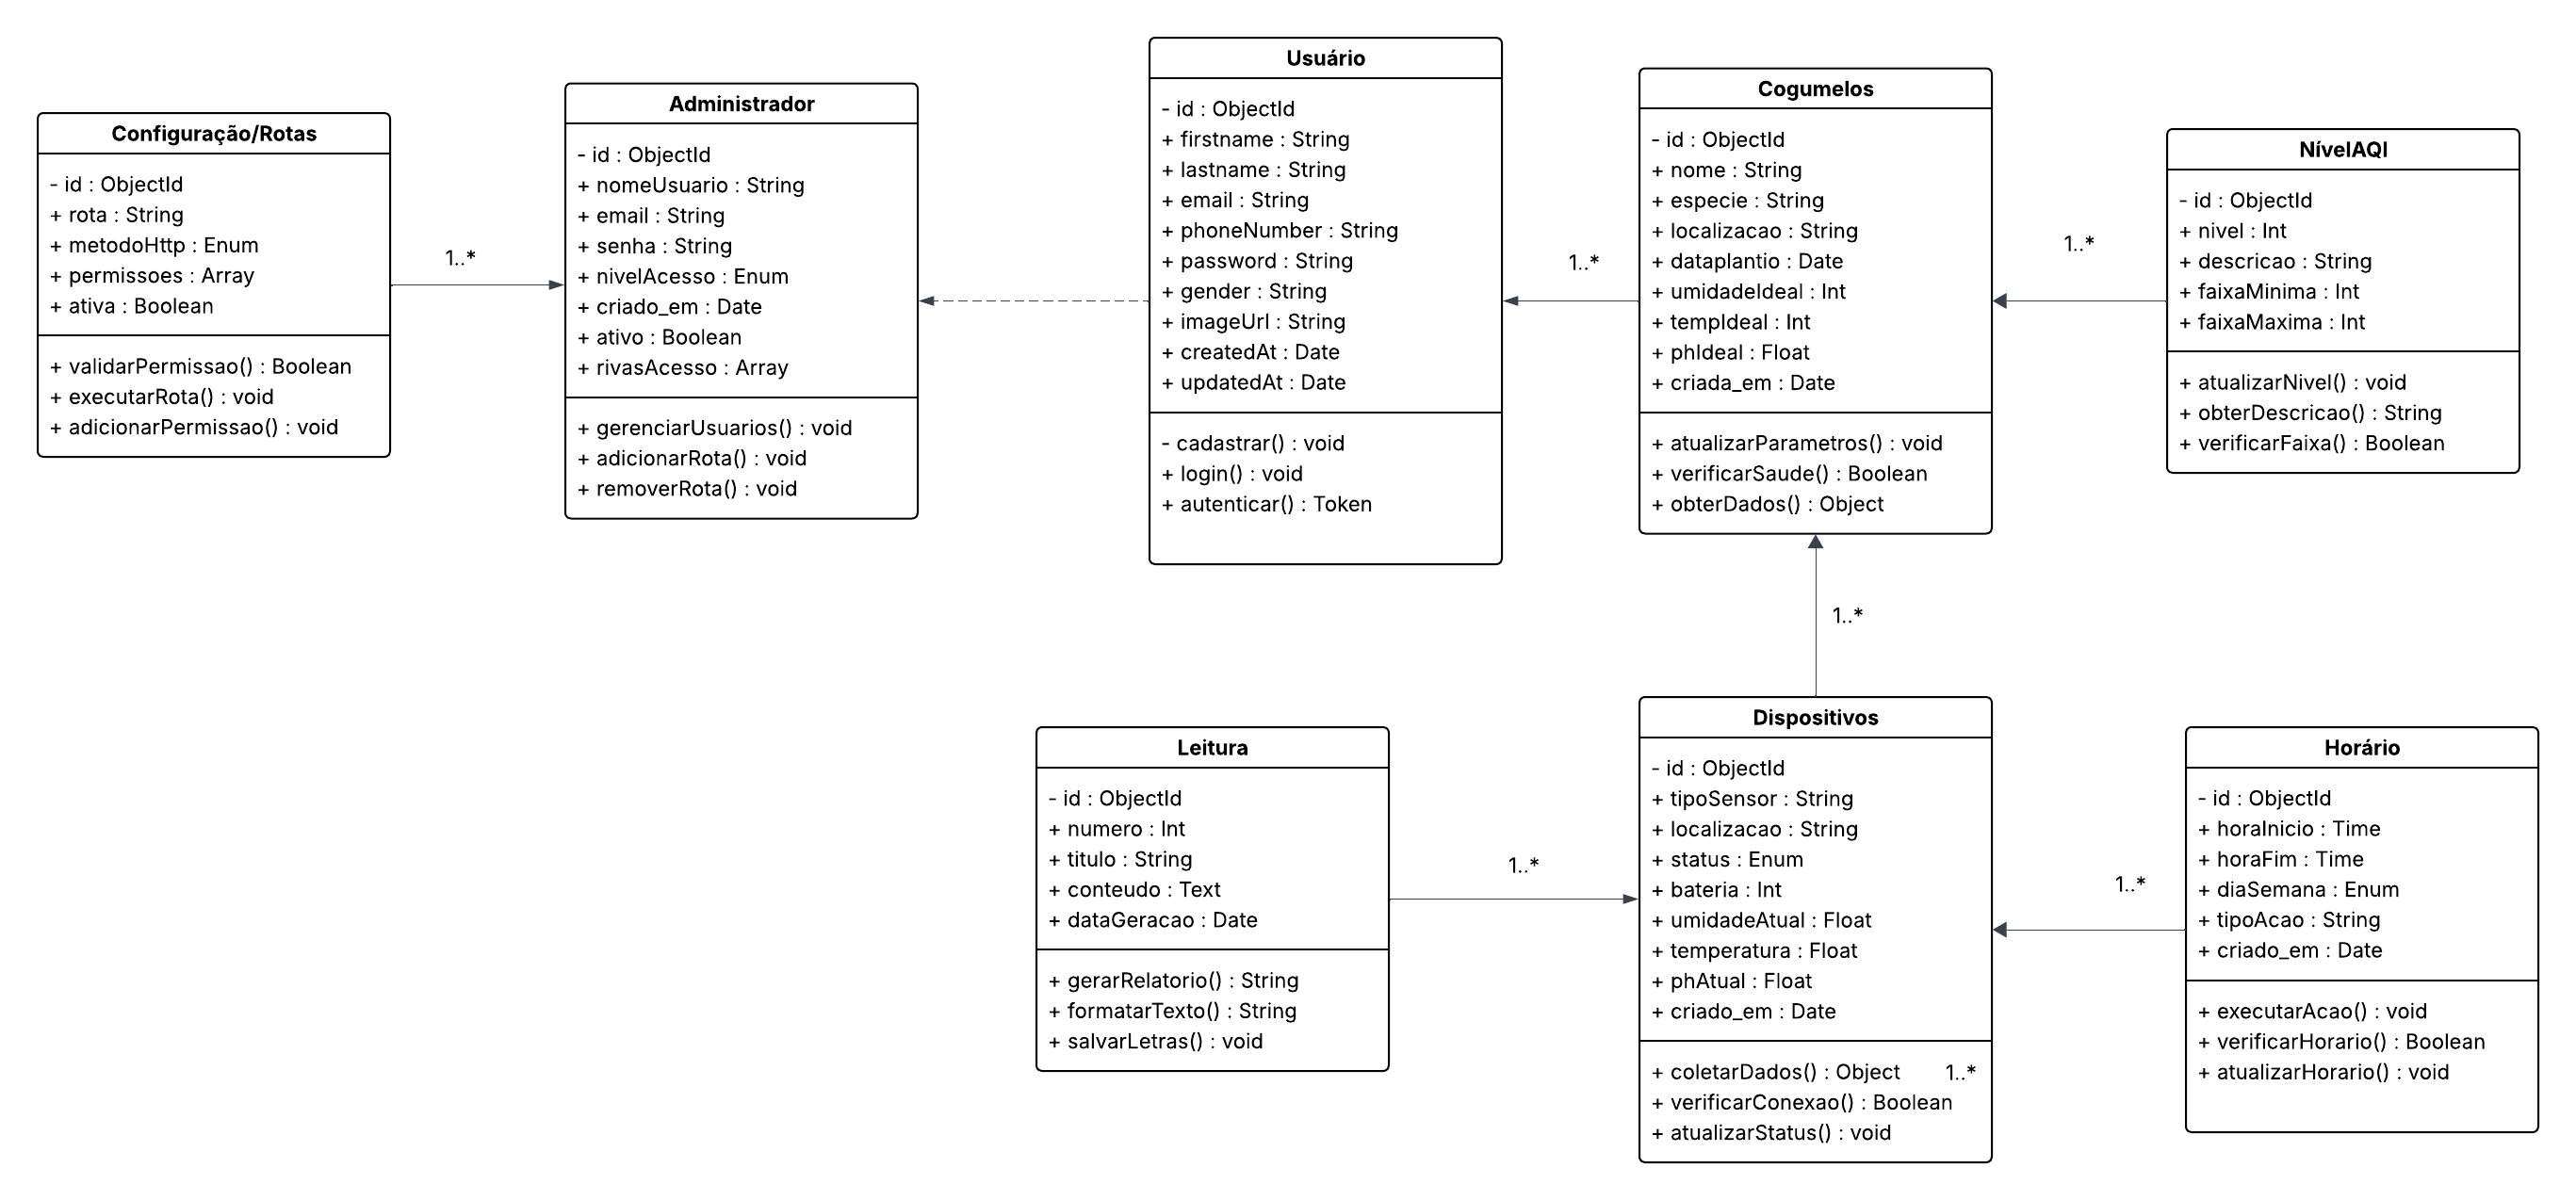
\includegraphics[
        width=0.8\textwidth,
        height=0.8\textheight,
        keepaspectratio
    ]{imgs/img_007.png}
    
    \caption{Diagrama de Classes -- Selene}
    \label{fig:classe}
\end{figure}

\subsection{Diagrama de Objetos}

O diagrama de objetos representa instâncias específicas das classes do sistema em determinado momento de execução, evidenciando os relacionamentos existentes entre os objetos da aplicação.

\begin{figure}[H]
\centering
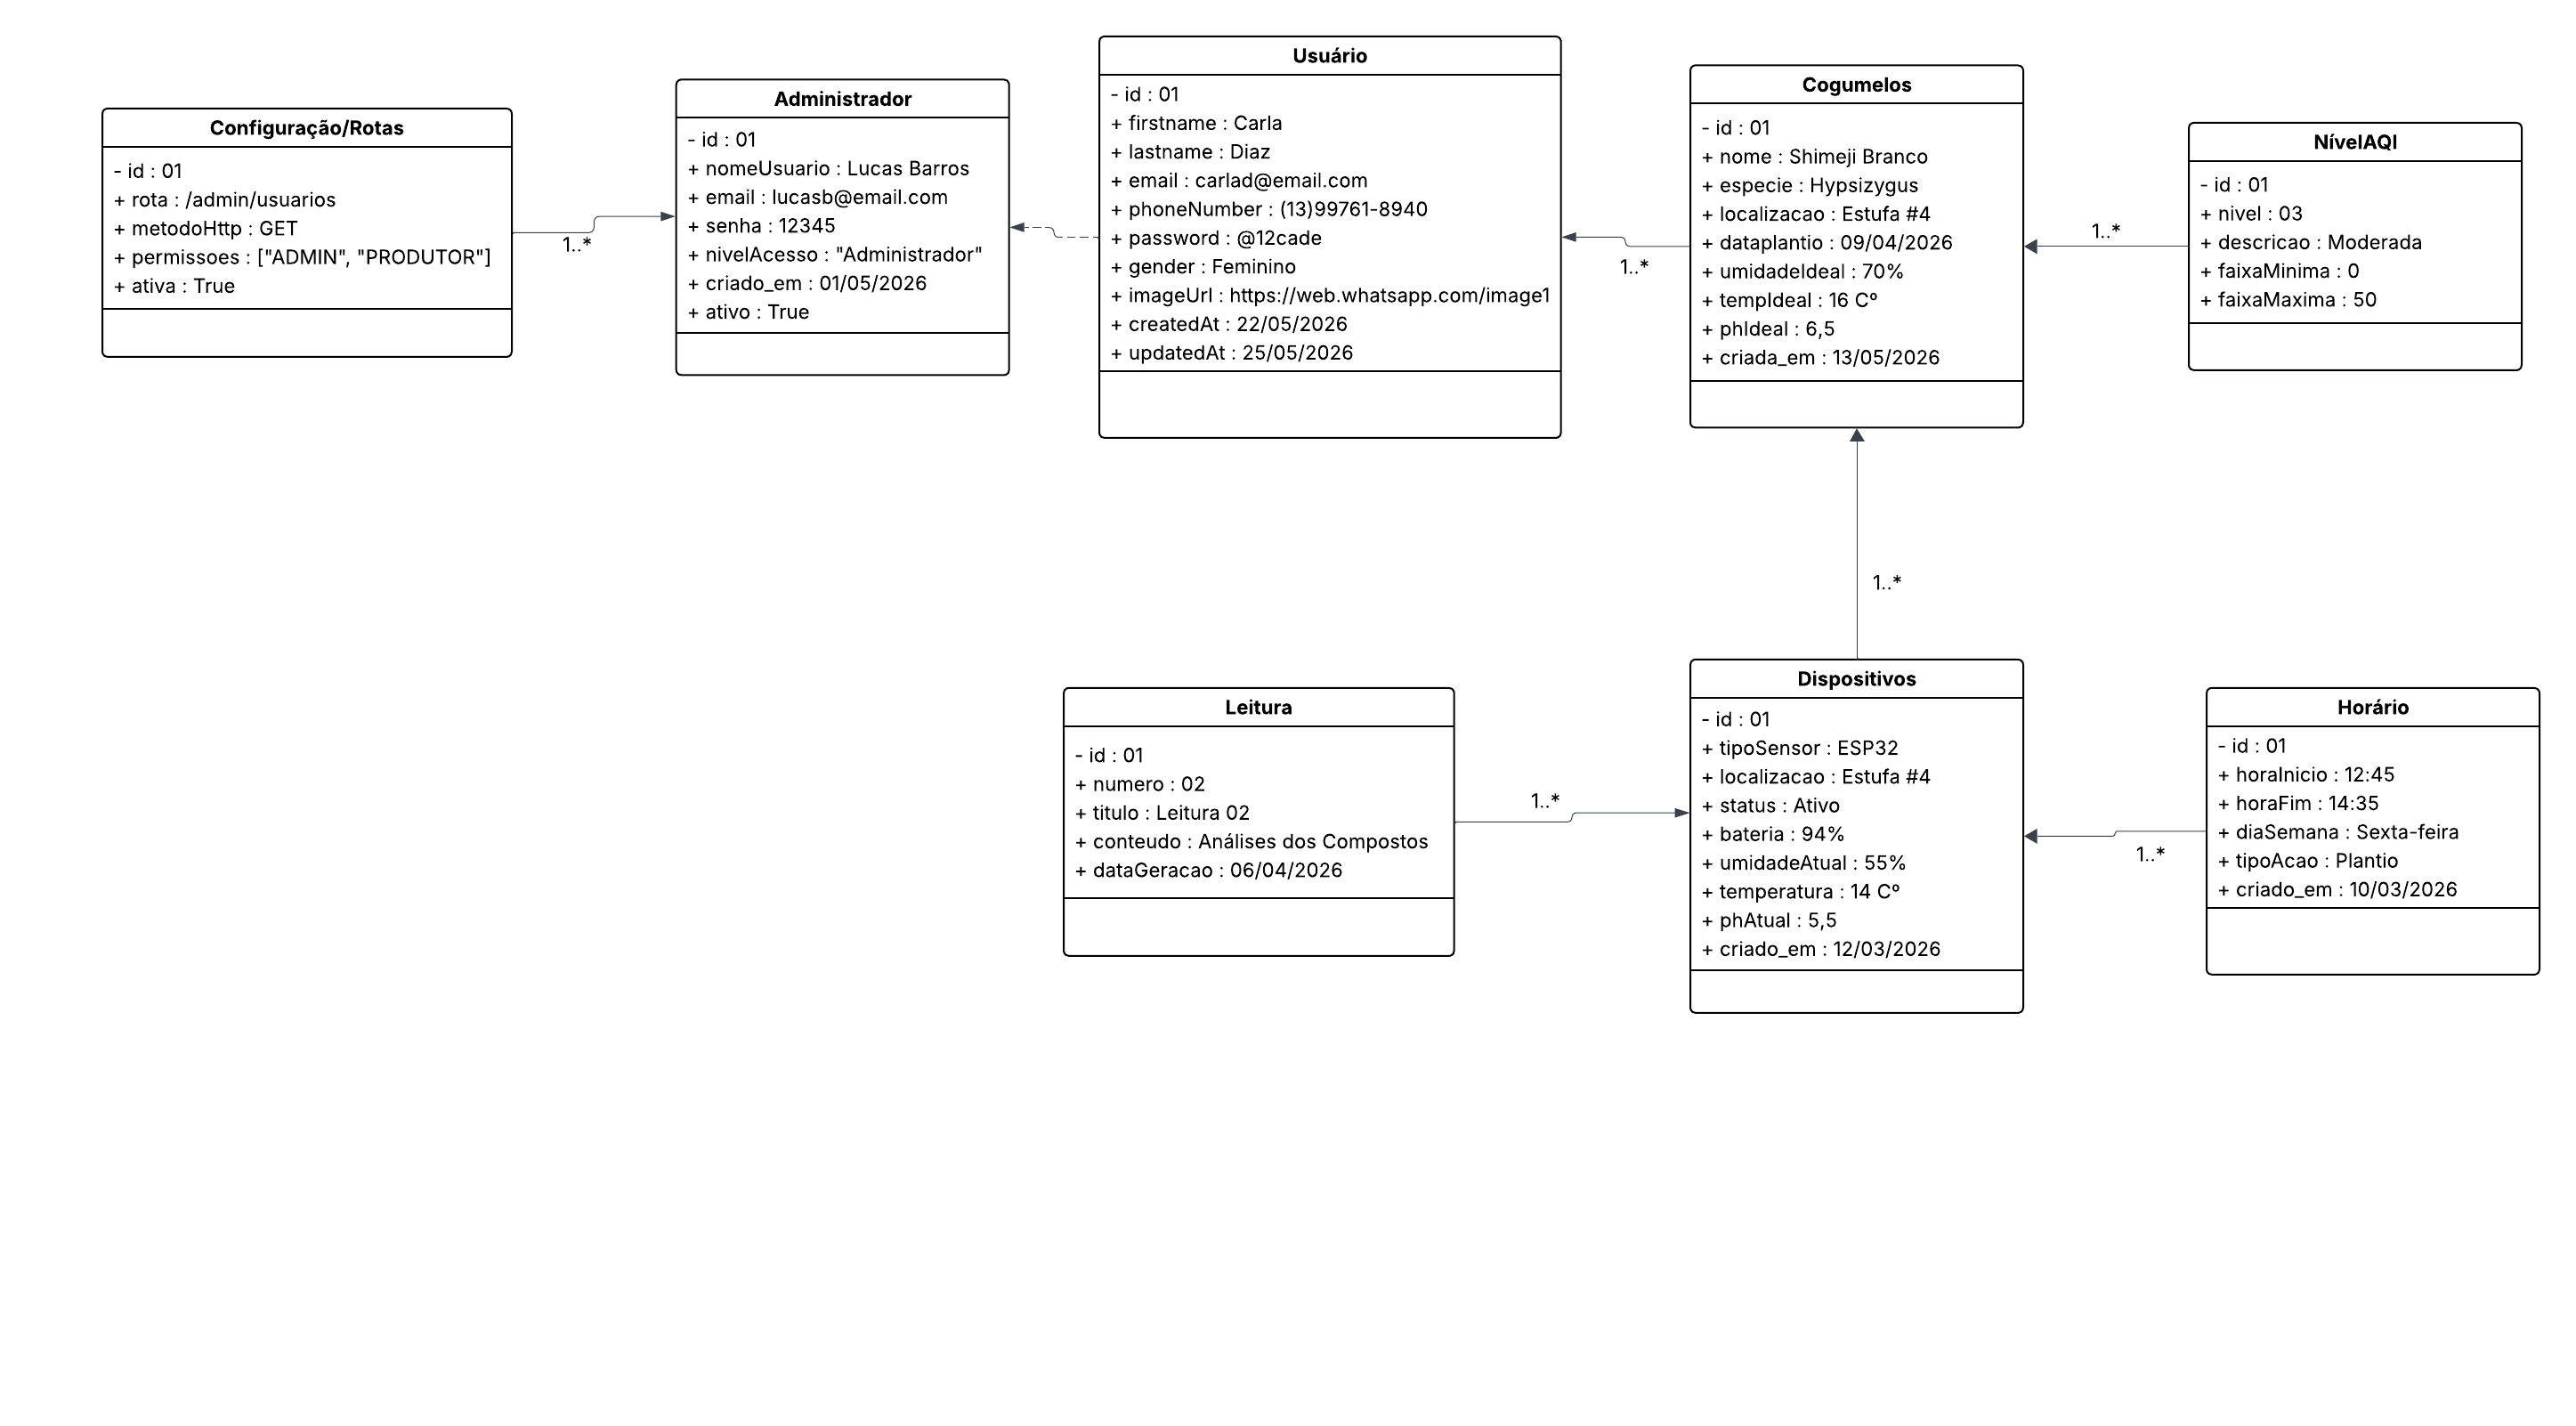
\includegraphics[width=\textwidth]{imgs/img_013.png}
\caption{Diagrama de Objetos -- Selene}
\label{fig:objetos}
\end{figure}

\subsection{Diagrama de Sequência}

O diagrama de sequência demonstra a interação entre os componentes do sistema ao longo do tempo, representando a troca de mensagens entre objetos e serviços.

\begin{figure}[H]
    \centering
    
    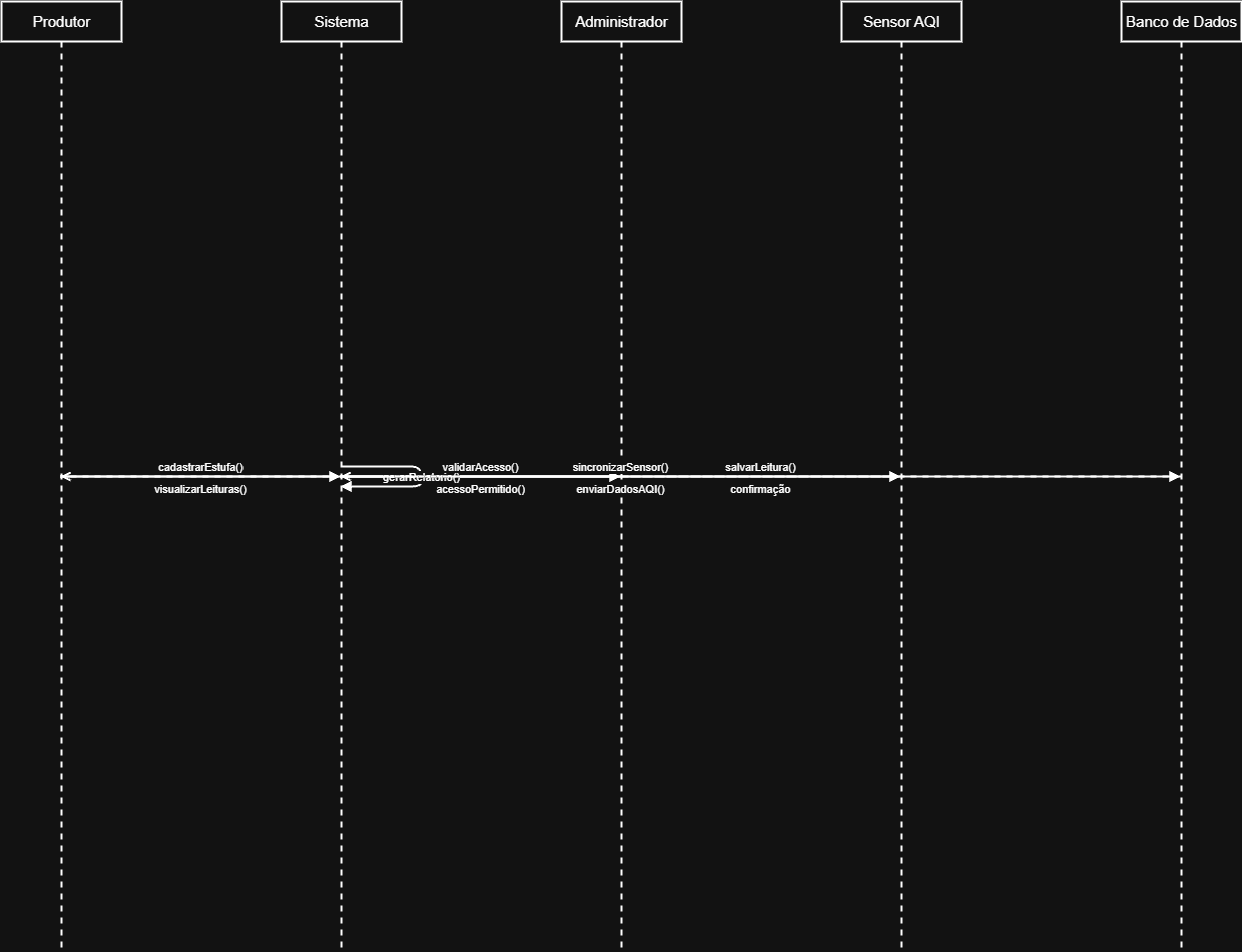
\includegraphics[
        width=0.7\textwidth,
        height=0.7\textheight,
        keepaspectratio
    ]{imgs/img_009.png}
    
    \caption{Diagrama de Sequência -- Selene}
    \label{fig:sequencia}
\end{figure}

\subsection{Diagrama de Atividades}

O diagrama de atividades representa os fluxos de processos e regras de negócio do sistema, descrevendo ações, decisões e caminhos de execução.

\begin{figure}[H]
    \centering
    
    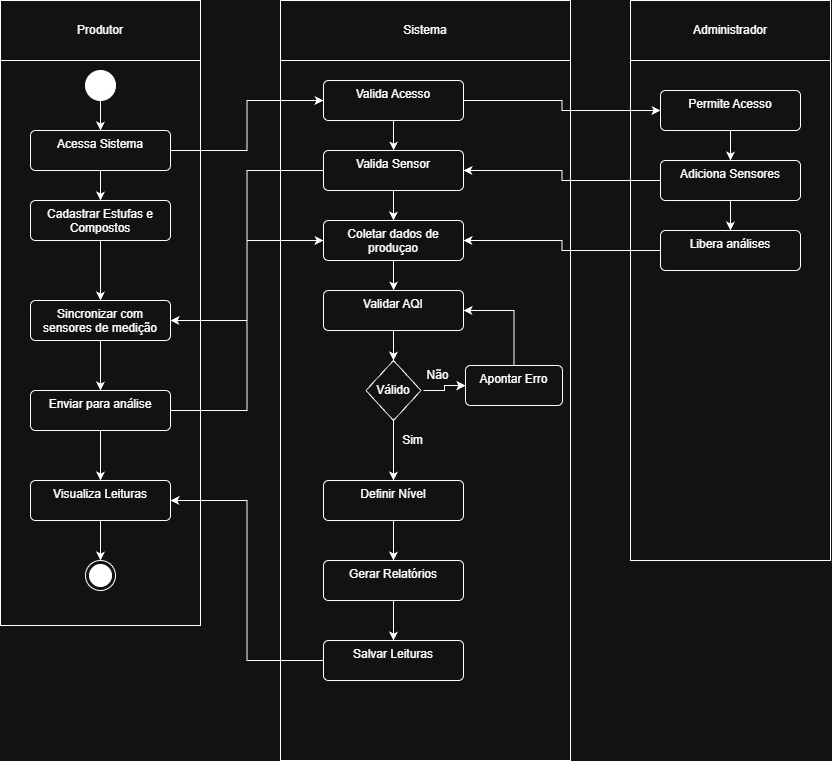
\includegraphics[
        width=0.7\textwidth,
        height=0.7\textheight,
        keepaspectratio
    ]{imgs/img_008.png}
    
    \caption{Diagrama de Atividades -- Selene}
    \label{fig:atividade}
\end{figure}

\subsection{Diagrama de Componentes}

O diagrama de componentes apresenta a organização estrutural dos módulos e componentes do sistema, destacando dependências e integrações entre as partes da aplicação.

\begin{figure}[H]
\centering
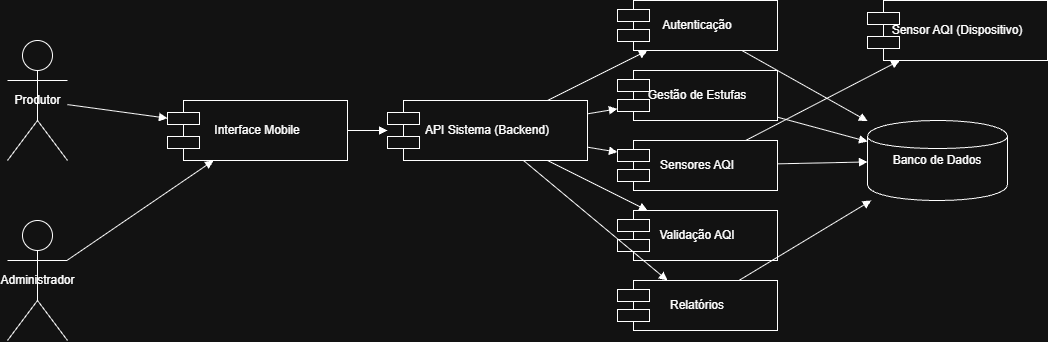
\includegraphics[width=\textwidth]{imgs/img_010.png}
\caption{Diagrama de Componentes -- Selene}
\label{fig:componentes}
\end{figure}

\subsection{Diagrama de Implantação}

O diagrama de implantação representa a arquitetura física do sistema, incluindo servidores, infraestrutura, banco de dados e distribuição dos componentes em ambiente de execução.

\begin{figure}[H]
    \centering
    
    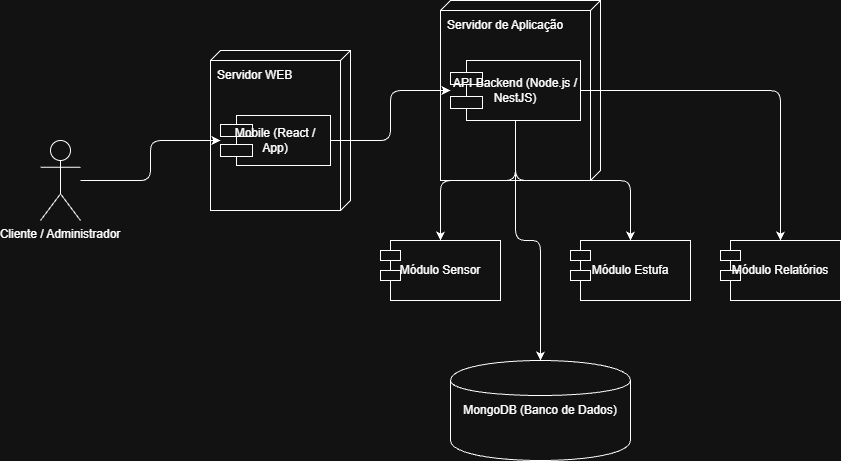
\includegraphics[
        width=0.7\textwidth,
        height=0.7\textheight,
        keepaspectratio
    ]{imgs/img_011.png}
    
    \caption{Diagrama de Implantação -- Selene}
    \label{fig:implantacao}
\end{figure}

\subsection{Diagrama de Estados}

O diagrama de estados demonstra os diferentes estados possíveis de uma entidade do sistema, bem como as transições decorrentes de eventos e ações.

\begin{figure}[H]
    \centering
    
    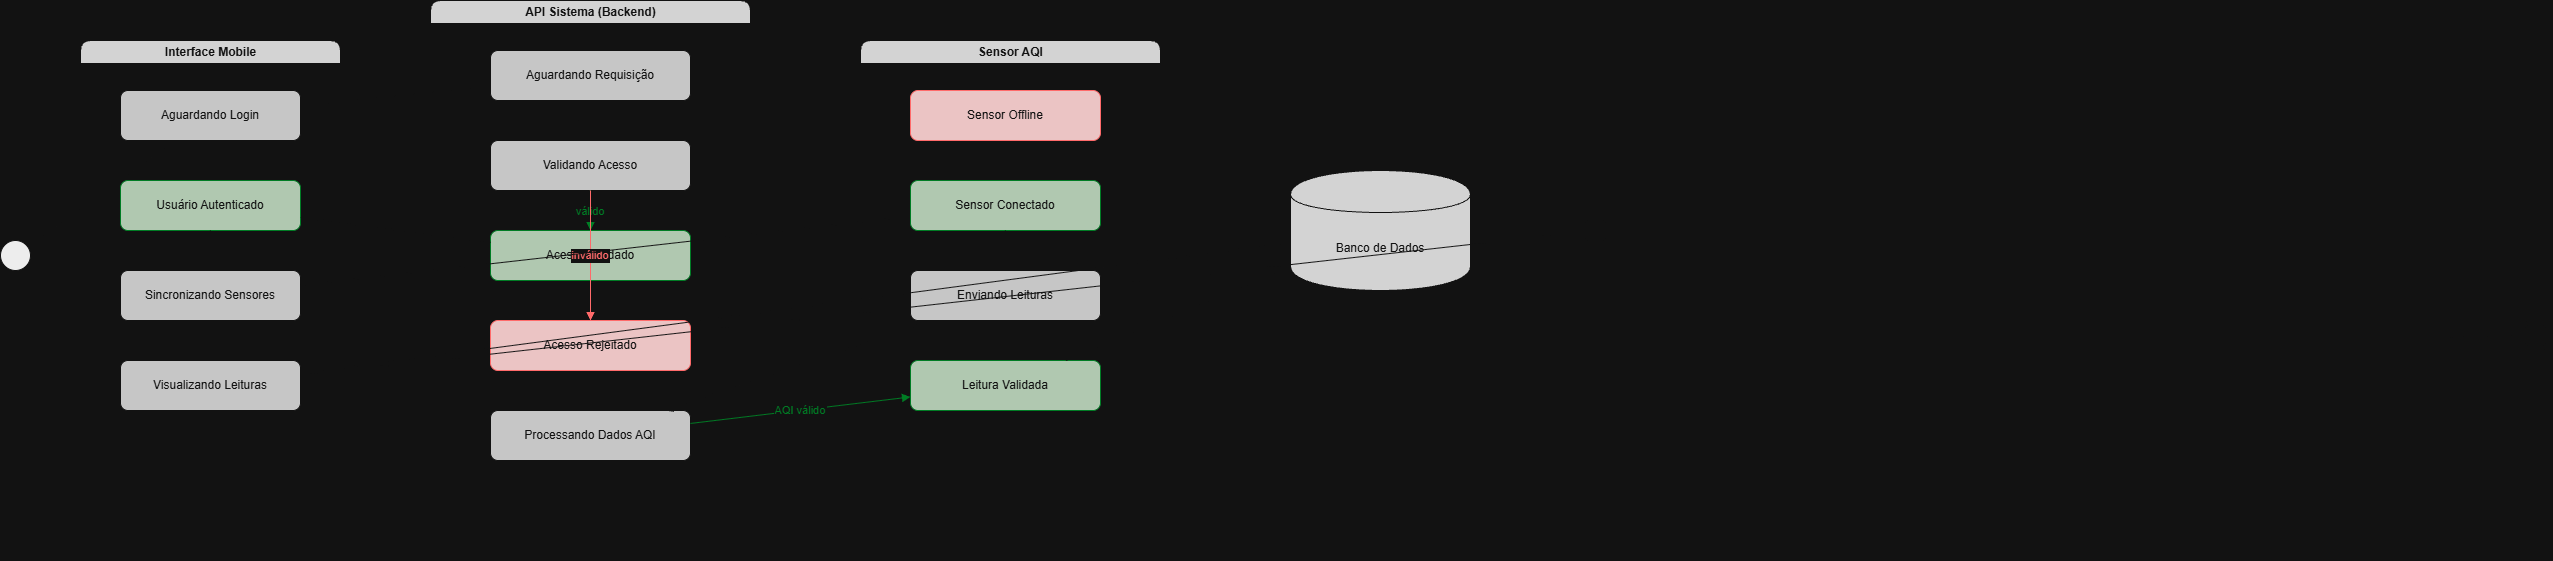
\includegraphics[
        width=0.9\textwidth,
        height=0.9\textheight,
        keepaspectratio
    ]{imgs/img_012.png}
    
    \caption{Diagrama de Estados -- Selene}
    \label{fig:estados}
\end{figure}

\subsection{Modelo de Banco de Dados}

O modelo de banco de dados apresenta a estrutura das entidades persistidas no sistema, seus atributos e relacionamentos, servindo como base para a implementação da camada de dados.

\begin{figure}[H]
\centering
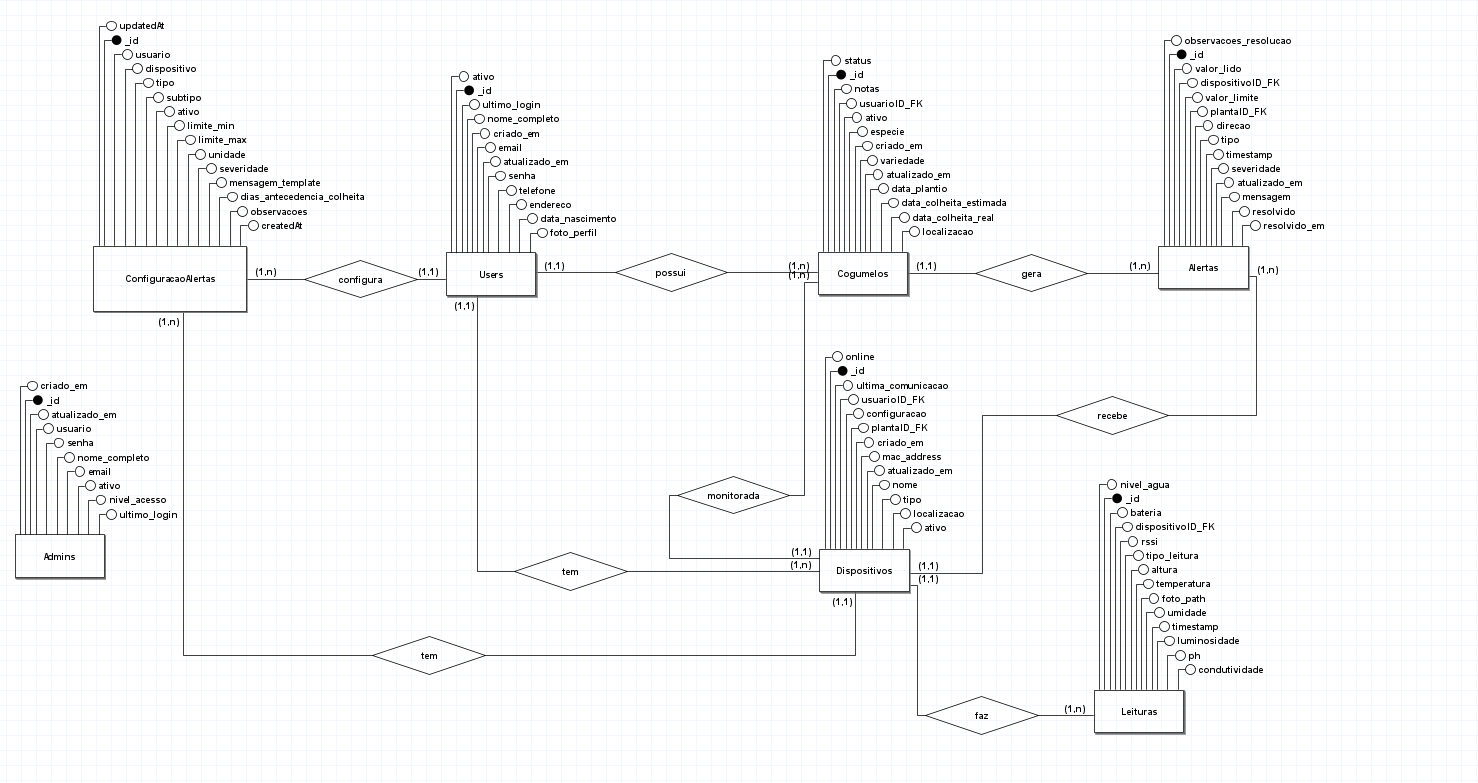
\includegraphics[width=\textwidth]{imgs/img_014.png}
\caption{Modelo de Banco de Dados -- Selene}
\label{fig:banco}
\end{figure}

% ===== DEVOPS =====
\section{DevOps: Infraestrutura, Automação e Entrega Contínua}

DevOps é uma cultura e um conjunto de práticas que integra desenvolvimento de software (Dev) e operações de TI (Ops), com foco em automação, colaboração e entrega contínua, sendo aplicada no software Selene para otimizar seus processos de desenvolvimento, implantação e manutenção, garantindo maior eficiência e confiabilidade do sistema.

\subsection{Pipeline CI/CD}

O pipeline de integração e entrega contínua é fundamental para a automação no software Selene, pois permite que alterações no código sejam testadas, validadas e implantadas de forma automática e consistente, reduzindo erros manuais, acelerando o ciclo de desenvolvimento e garantindo maior estabilidade nas versões disponibilizadas.

\begin{figure}[H]
    \centering
    
    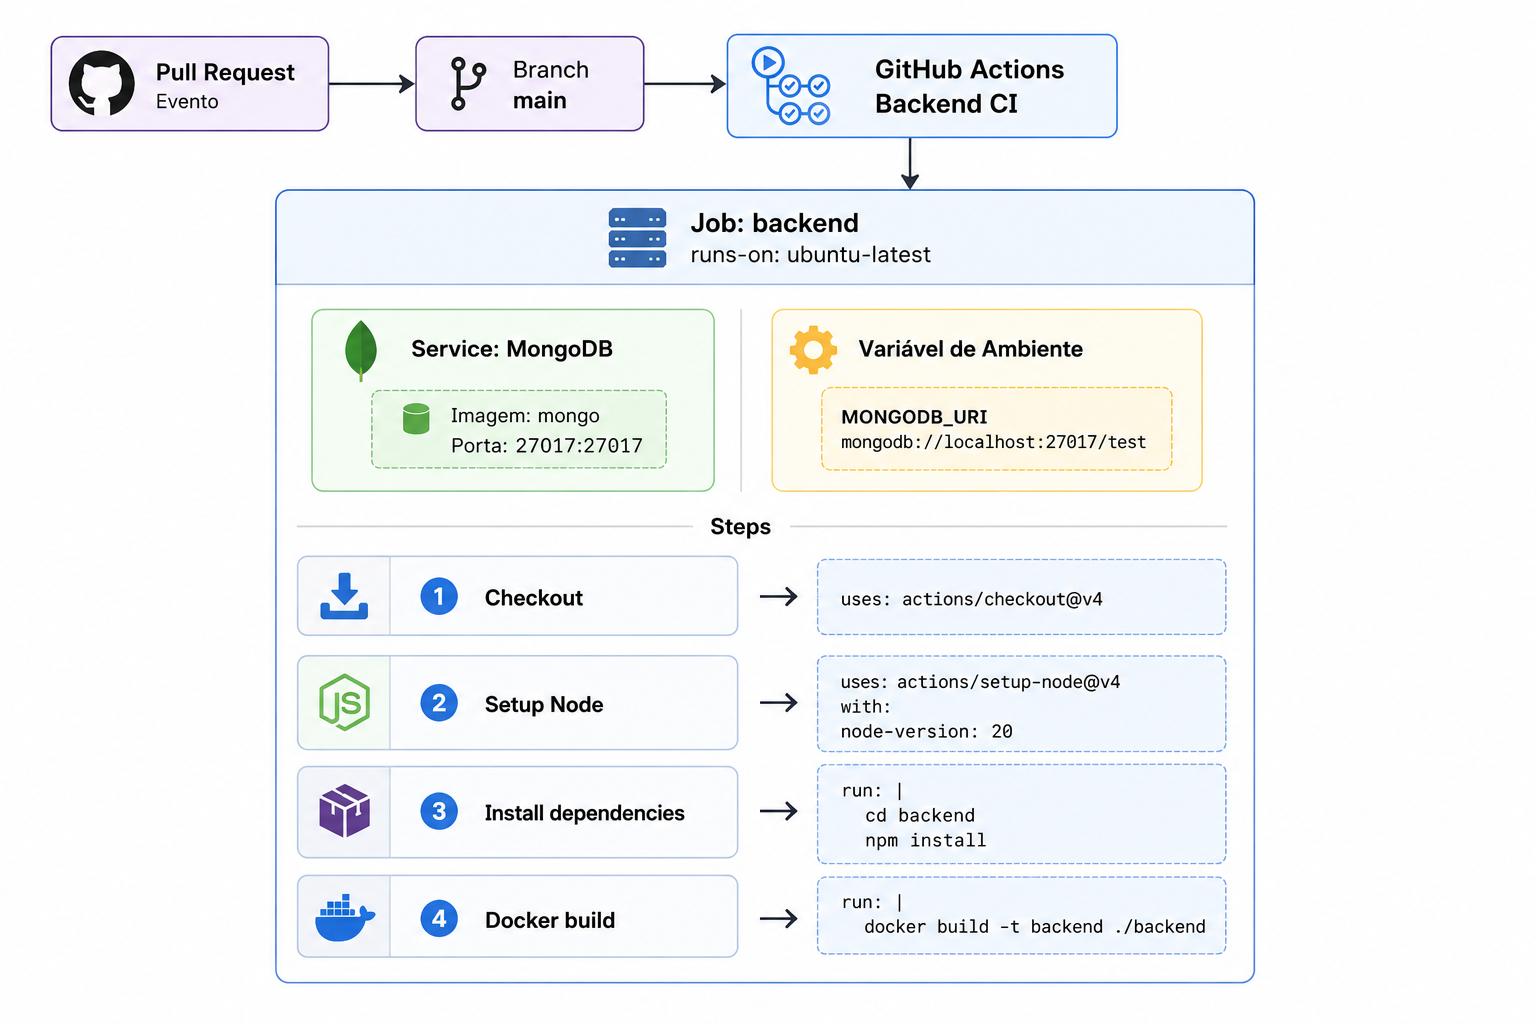
\includegraphics[
        width=0.7\textwidth,
        height=0.7\textheight,
        keepaspectratio
    ]{imgs/img_015.png}
    
    \caption{Modelo CI/CD -- Selene}
    \label{fig:ci}
\end{figure}

\subsection{Configuração CI/CD}

Arquivo de CI/CD do Selene (selene-ci.yml) e GitHub Actions:

\begin{verbatim}
name: Backend CI
on:
  pull_request:
    branches:
      - main

jobs:
  backend:
    runs-on: ubuntu-latest

    services:
      mongo:
        image: mongo
        ports:
          - 27017:27017

    env:
      MONGODB_URI: mongodb://localhost:27017/test

    steps:
      - name: Checkout
        uses: actions/checkout@v4

      - name: Setup Node
        uses: actions/setup-node@v4
        with:
          node-version: 20

      - name: Install dependencies
        run: |
          cd backend
          npm install

      - name: Docker build
        run: |
          docker build -t backend ./backend


name: Docker Publish

on:
  push:
    branches:
      - main

jobs:
  docker:
    runs-on: ubuntu-latest

    steps:
      - name: Checkout
        uses: actions/checkout@v4

      - name: Login DockerHub
        uses: docker/login-action@v3
        with:
          username: ${{ secrets.DOCKER_USERNAME }}
          password: ${{ secrets.DOCKER_PASSWORD }}

      - name: Build Docker image
        run: |
          docker build \
          -t ${{ secrets.DOCKER_USERNAME }}/selene-backend:latest \
          -t ${{ secrets.DOCKER_USERNAME }}/selene-backend:${{ github.run_id }} \
          ./backend

      - name: Push latest
        run: |
          docker push ${{ secrets.DOCKER_USERNAME }}/selene-backend:latest

      - name: Push version tag
        run: |
          docker push ${{ secrets.DOCKER_USERNAME }}/selene-backend:${{ github.run_id }}
\end{verbatim}

\subsection{Infraestrutura como Código}

\begin{table}[H]
\centering
\caption{Ferramentas DevOps Utilizadas no Projeto}
\label{tab:devops-tools}

\renewcommand{\arraystretch}{1.5} % Espaçamento entre linhas

\begin{tabular}{|>{\centering\arraybackslash}m{4cm}
                |>{\centering\arraybackslash}m{4cm}
                |m{8cm}|}
\hline

\rowcolor[HTML]{D9EAF7}
\textbf{Categoria} &
\textbf{Ferramenta} &
\textbf{Finalidade} \\

\hline

Controle de Versão &
Git + GitHub &
Utilizados para realizar o controle de versão do código-fonte, permitindo o gerenciamento das alterações realizadas no projeto, colaboração entre desenvolvedores e armazenamento seguro do repositório em nuvem. \\

\hline

CI/CD &
GitHub Actions &
Responsável pela automação dos processos de integração contínua e entrega contínua, executando tarefas como build, testes automatizados e deploy da aplicação de forma padronizada e eficiente. \\

\hline

Containerização &
Docker &
Empregado para criar e gerenciar contêineres da aplicação, garantindo padronização do ambiente de desenvolvimento, testes e produção, além de facilitar a implantação do sistema em diferentes servidores. \\

\hline

\end{tabular}
\end{table}

\subsection{Infraestrutura do Sistema}

Esta seção descreve o funcionamento do sistema Selene em diferentes ambientes e plataformas.

\subsubsection{Arquitetura de Rede}

\begin{table}[H]
\centering
\caption{Componentes de Infraestrutura do Sistema}
\label{tab:infrastructure}

\renewcommand{\arraystretch}{1.5}

\begin{tabular}{|>{\centering\arraybackslash}m{4cm}|m{10cm}|}
\hline

\rowcolor[HTML]{D9EAF7}
\textbf{Componente} & \textbf{Descrição} \\

\hline

\textbf{Rede Local (LAN)} & 
A infraestrutura de rede local é utilizada para garantir a comunicação interna entre os dispositivos e servidores da organização. Além disso, são realizados backups locais diários em um servidor dedicado, assegurando maior disponibilidade e recuperação de dados em caso de falhas ou perdas de informação. \\

\hline

\textbf{Cloud (Nuvem)} & 
Os serviços em nuvem são utilizados para hospedagem e gerenciamento do banco de dados por meio do MongoDB Atlas, proporcionando alta disponibilidade, escalabilidade e segurança. O ambiente também conta com mecanismos de auto-scaling, permitindo que os recursos sejam ajustados automaticamente conforme a demanda do sistema. \\

\hline

\textbf{Dispositivos Móveis} & 
A integração com dispositivos móveis é realizada através de uma API REST, possibilitando a comunicação entre aplicações mobile e o servidor principal. O sistema também utiliza notificações push para envio de atualizações, alertas e informações em tempo real aos usuários. \\

\hline

\textbf{Segurança} & 
A camada de segurança do sistema utiliza autenticação baseada em JWT e OAuth 2.0 para controle de acesso e proteção das rotas da aplicação. Além disso, são aplicadas técnicas de criptografia para proteção de dados sensíveis, juntamente com monitoramento contínuo de acessos e geração de logs de auditoria para rastreabilidade e conformidade. \\

\hline

\end{tabular}
\end{table}

\subsubsection{Diagrama de Infraestrutura}

Para ilustrar como os componentes se conectam:

\begin{figure}[H]
    \centering
    
    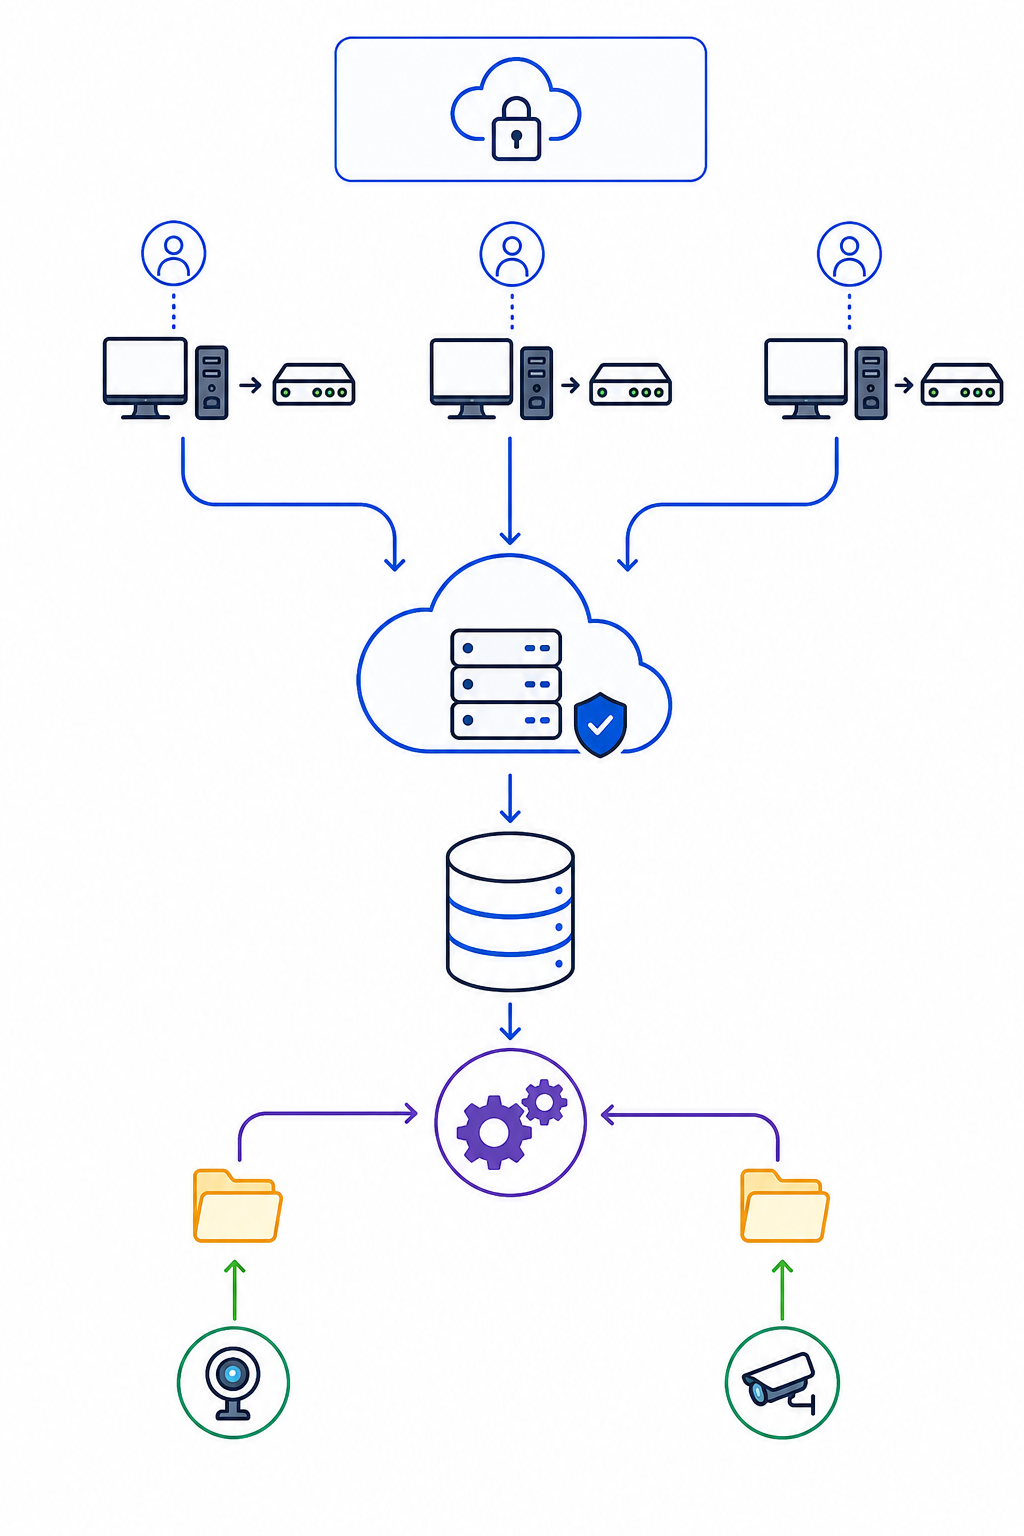
\includegraphics[
        width=0.7\textwidth,
        height=0.7\textheight,
        keepaspectratio
    ]{imgs/img_016.png}
    
    \caption{Diagrama Redes -- Selene}
    \label{fig:redes}
\end{figure}

\begin{itemize}
    \item \textbf{Camada de Segurança / Autenticação (Cloud):} Responsável por proteger o acesso ao sistema, garantindo autenticação e criptografia das comunicações.
    
    \item \textbf{Usuários:} Acessam a aplicação via mobile, utilizando conexão segura.
    
    \item \textbf{Manutenção:} Dispositivos desktop que se conectam ao backend através de rede autenticada.
    
    \item \textbf{Gateway / Cluster de Backend:} Camada central de serviços que recebe todas as requisições dos usuários e direciona o tráfego para os serviços internos.
    
    \item \textbf{Banco de Dados Central:} Responsável pelo armazenamento estruturado das informações do sistema, garantindo persistência e consistência dos dados.
    
    \item \textbf{Camada de Processamento (Engine / Microserviços):} Realiza o processamento das regras de negócio e orquestra as operações do sistema.
    
    \item \textbf{Armazenamento de Arquivos:} Repositório para documentos, imagens e dados não estruturados (equivalente a storage tipo S3).
    
    \item \textbf{Integração com Dispositivos de Entrada:} Inclui fontes de dados externas que alimentam o sistema:
    \begin{itemize}
        \item Câmeras de monitoramento: Enviam dados visuais para processamento e armazenamento.
        \item Webcams / dispositivos de captura: Fornecem entrada de mídia para o sistema.
        \item Serviços de Arquivos (Pastas/Uploads): Fontes de dados como uploads de usuários e integrações externas.
    \end{itemize}
\end{itemize}

\subsection{Arquitetura de Deploy}

Arquitetura de deployment:

\begin{figure}[H]
\centering
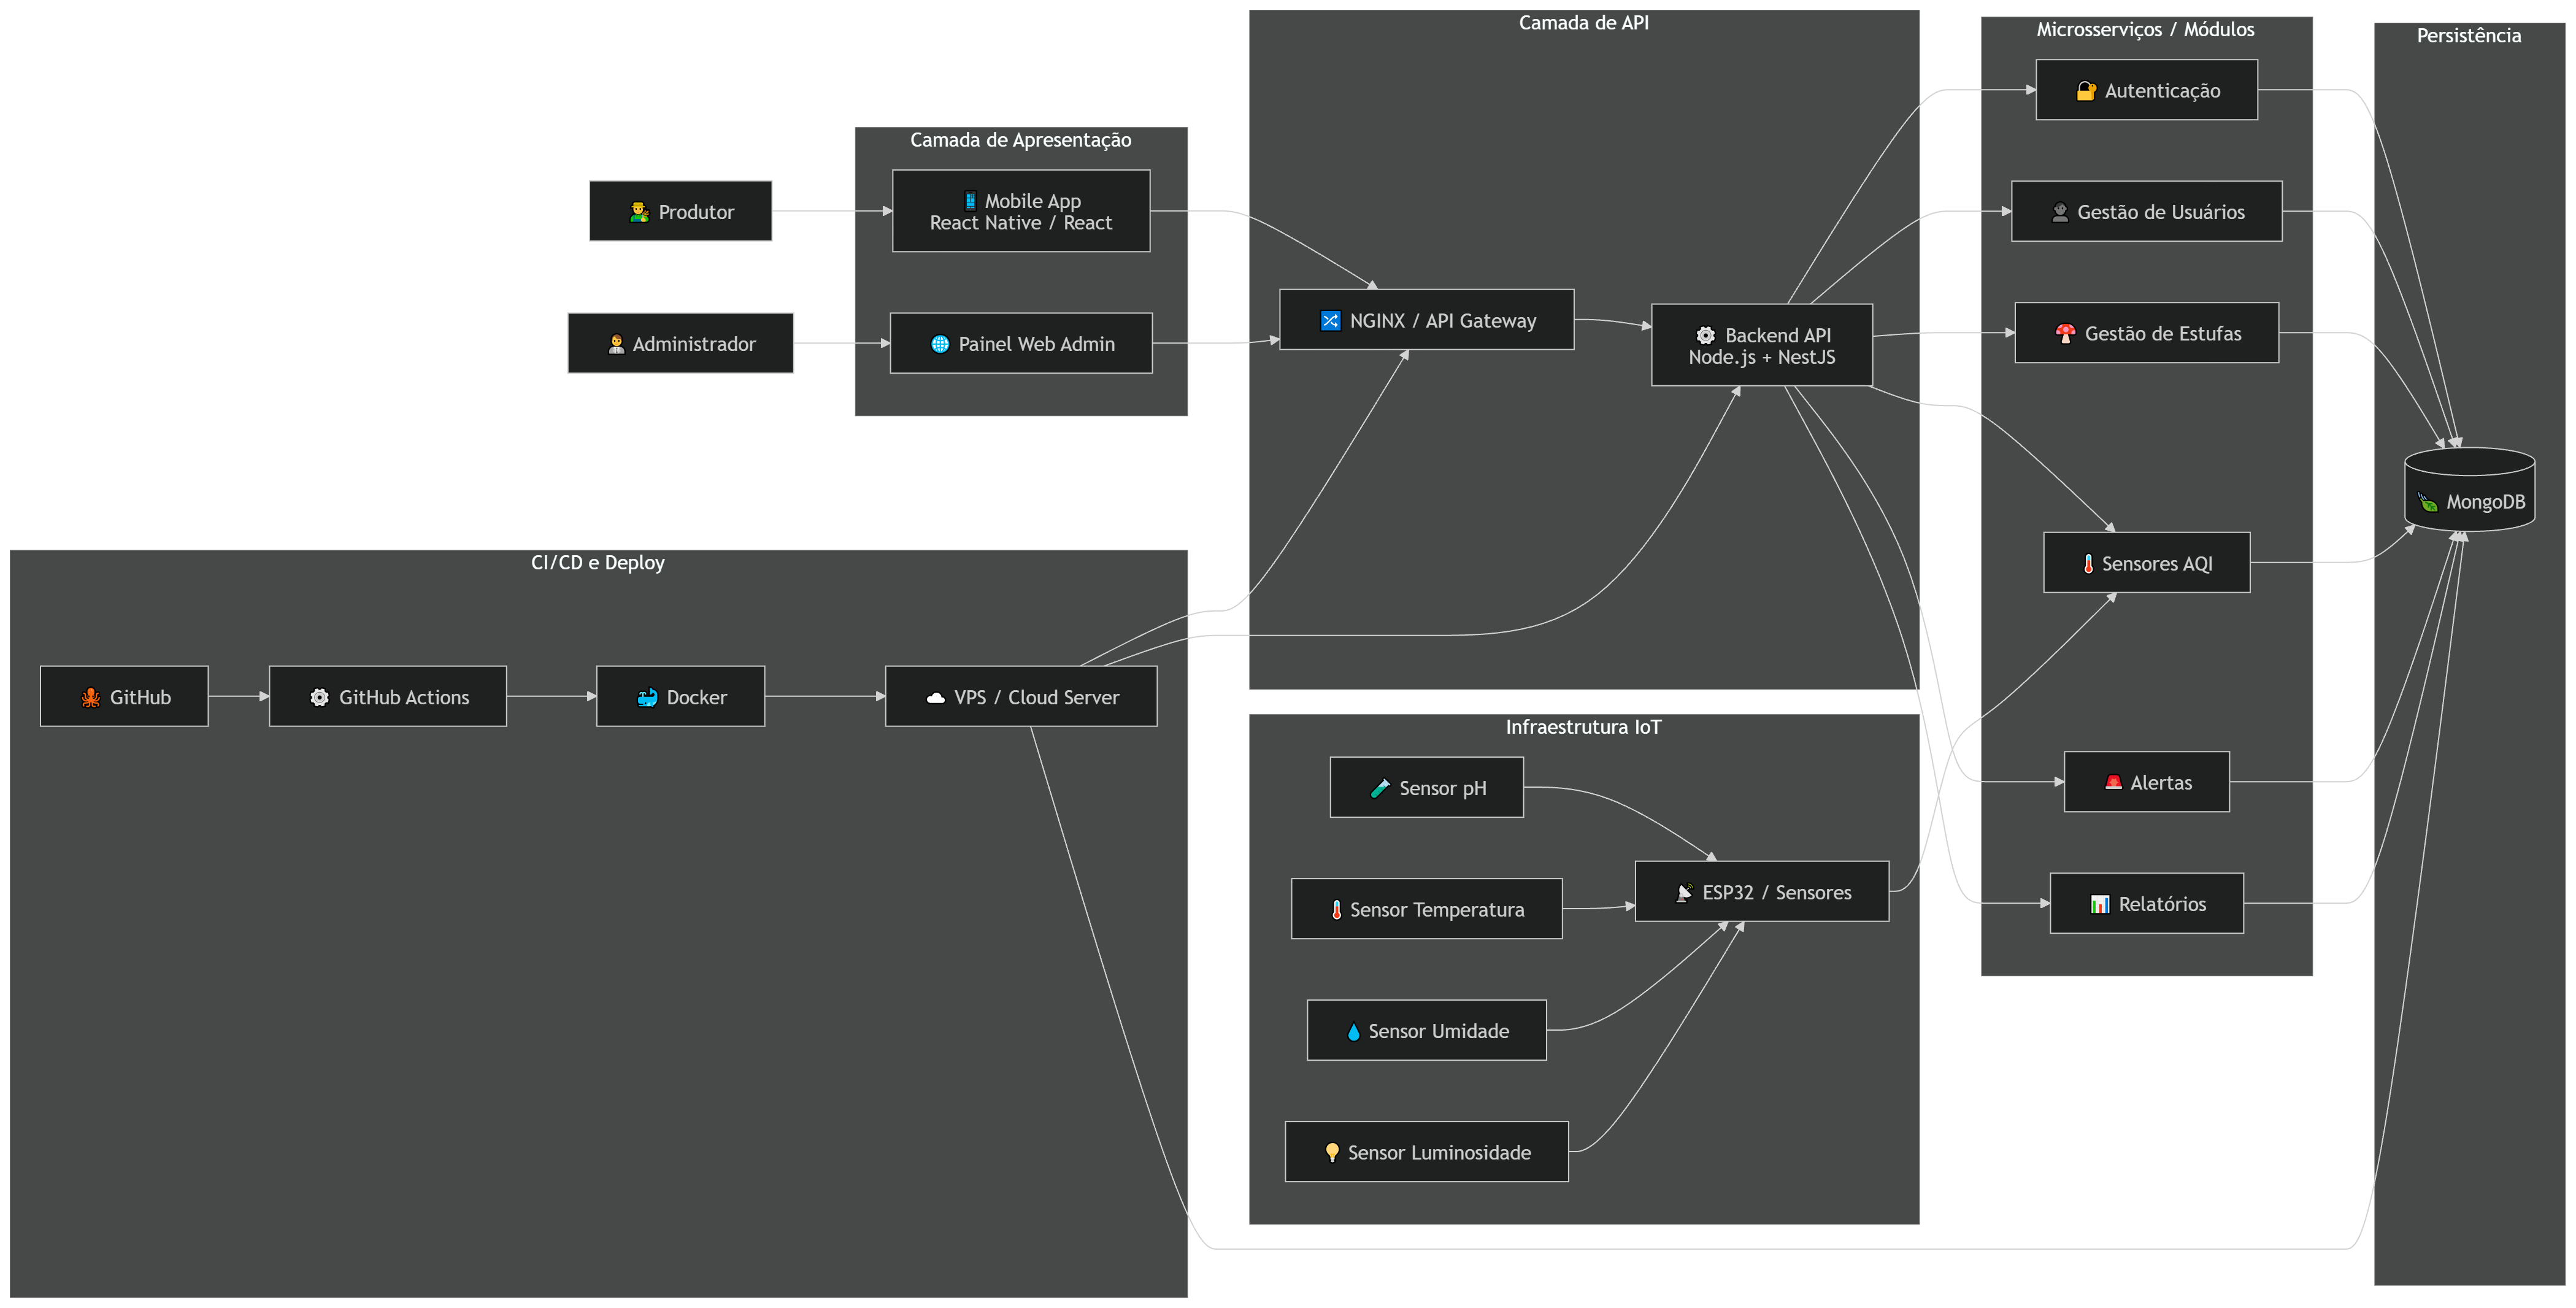
\includegraphics[width=\textwidth]{imgs/img_017.png}
\caption{Deployment - Selene}
\label{fig:deploy}
\end{figure}

\subsection{Métricas Propostas}

A seguir são apresentadas as métricas SRE/DevOps:
\begin{table}[H]
\centering
\scriptsize % diminui o tamanho da tabela

\begin{tabular}{|p{1.8cm}|p{1.8cm}|p{2.8cm}|p{3.5cm}|}
\hline
\textbf{Métrica} & \textbf{SLO} & \textbf{SLI} & \textbf{Justificativa} \\
\hline

Disponibilidade (Uptime) & 99\% -- 99.5\% &
Tempo de atividade medido por health checks do sistema &
Garante operação contínua do monitoramento ambiental, reduzindo riscos ao cultivo. \\
\hline

Tempo de Resposta & $\leq 1s$ &
Tempo entre leitura do sensor, processamento da IA e ação do atuador &
Essencial para resposta rápida a variações ambientais críticas. \\
\hline

Taxa de Erro & $< 0.5\%$ &
Erros totais em sensores, IA ou execução de comandos &
Evita decisões incorretas que impactem diretamente o cultivo. \\
\hline

Throughput & 100 -- 500 req/s &
Requisições de sensores processadas por segundo &
Compatível com múltiplos sensores distribuídos em estufas IoT. \\
\hline

Deploy Frequency & 1 -- 3 por semana &
Número de deploys bem-sucedidos em produção &
Permite atualizações seguras sem comprometer estabilidade do ambiente físico. \\
\hline

Lead Time & 2 -- 6 horas &
Tempo entre commit e deploy em produção &
Equilibra velocidade de entrega com validação de estabilidade do sistema. \\
\hline

MTTR & 30 -- 60 minutos &
Tempo médio de recuperação após falha &
Minimiza impactos no controle ambiental do cultivo. \\
\hline

Precisão da IA & $\geq 90\%$ &
Taxa de acerto das decisões da rede neural &
Garante confiabilidade nas ações automáticas do sistema. \\
\hline

Freshness dos Dados & $\leq 10s$ &
Idade máxima dos dados usados pela IA &
Assegura decisões baseadas em dados atualizados do ambiente. \\
\hline

Latência IoT & $\leq 2s$ &
Tempo entre sensor físico e ingestão no sistema &
Essencial para integração entre mundo físico e sistema de IA. \\
\hline

\end{tabular}

\caption{Métricas SRE/DevOps -- SELENE}
\label{tab:sre}
\end{table}

\newpage
\section*{Conclusão}

Este documento consolida os principais artefatos de engenharia de software necessários para a especificação, organização e governança do sistema \textbf{Selene}, uma plataforma inteligente baseada em Inteligência Artificial e Internet das Coisas (IoT) voltada ao monitoramento e controle da produção de cogumelos em ambientes controlados.

A estrutura apresentada permite documentar de forma integrada tanto os aspectos estratégicos quanto técnicos do sistema, garantindo rastreabilidade entre requisitos de negócio, arquitetura, implementação e operação em produção.

Os artefatos descritos incluem:

\begin{itemize}
    \item \textbf{CANVAS:} Estruturação do modelo de negócio do sistema Selene, definindo proposta de valor, stakeholders e viabilidade da solução de monitoramento inteligente para cultivo de cogumelos.
    
    \item \textbf{SWOT:} Análise estratégica das forças, fraquezas, oportunidades e ameaças associadas à adoção de tecnologias de IA e IoT no contexto agrícola controlado.
    
    \item \textbf{UX/UI:} Definição da experiência do usuário e interfaces operacionais do sistema, permitindo interação eficiente com dados ambientais em tempo real e decisões automatizadas.
    
    \item \textbf{Website da Equipe:} Desenvolvimento do site institucional do grupo responsável pelo projeto Selene, com o objetivo de apresentar o time, documentação, progresso do sistema e informações relevantes do desenvolvimento.
    
    \item \textbf{Diagramas UML:} Modelagem estrutural e comportamental do sistema, representando componentes, fluxos de dados e interações entre IA, sensores IoT e módulos de controle.
    
    \item \textbf{DevOps:} Definição da infraestrutura de entrega contínua, automação, monitoramento e confiabilidade do sistema, incluindo práticas de Site Reliability Engineering (SRE) aplicadas ao ambiente de produção agrícola.
\end{itemize}
\end{document}
